\documentclass[11pt,xcolor={dvipsnames}, aspectratio=169]{beamer}
\usetheme[
%%% option passed to the outer theme
%    progressstyle=fixedCircCnt,   % fixedCircCnt, movingCircCnt (moving is deault)
  ]{Feather}
  
% If you want to change the colors of the various elements in the theme, edit and uncomment the following lines

% Change the bar colors:
\setbeamercolor{Feather}{fg=NavyBlue!20,bg=NavyBlue}
%
%% Change the color of the structural elements:
\setbeamercolor{structure}{fg=NavyBlue}
%
%% Change the frame title text color:
\setbeamercolor{frametitle}{fg=black!5}
%
%% Change the normal text colors:
\setbeamercolor{normal text}{fg=black!75,bg=gray!5}
%
%%% Change the block title colors
\setbeamercolor{block title}{use=Feather,bg=Feather.fg, fg=black!90} 


% Change the logo in the upper right circle:
%\renewcommand{\logofile}{example-grid-100x100pt} 
%% This is an image that comes with the LaTeX installation
% Adjust scale of the logo w.r.t. the circle; default is 0.875
% \renewcommand{\logoscale}{0.55}

% Change the background image on the title and final page.
% It stretches to fill the entire frame!
% \renewcommand{\backgroundfile}{example-grid-100x100pt}

%-------------------------------------------------------
% INCLUDE PACKAGES
%-------------------------------------------------------

\usepackage{amsmath}
\usepackage{amsfonts}
\usepackage{pgfplots}
\usepackage{filecontents}
\usepackage{caption}
\usepackage{subcaption}

% If you want to change the colors of the various elements in the theme, edit and uncomment the following lines

% Change the bar colors:
%\setbeamercolor{Feather}{fg=red!20,bg=red}

% Change the color of the structural elements:
%\setbeamercolor{structure}{fg=red}

% Change the frame title text color:
%\setbeamercolor{frametitle}{fg=blue}

% Change the normal text color background:
%\setbeamercolor{normal text}{fg=black,bg=gray!10}

%-------------------------------------------------------
% INCLUDE PACKAGES
%-------------------------------------------------------

\usepackage[utf8]{vietnam}
\usepackage{amsmath}
\usepackage{algorithm}
\usepackage[noend]{algpseudocode}
\usepackage{geometry}
\usepackage{float}
\usepackage{helvet}
% \usepackage{helvet}

%% Load different font packages to use different fonts
%% e.g. using Linux Libertine, Linux Biolinum and Inconsolata
% \usepackage{libertine}
% \usepackage{zi4}

%% e.g. using Carlito and Caladea


%% e.g. using Venturis ADF Serif and Sans
% \usepackage{venturis}

%-------------------------------------------------------
% DEFFINING AND REDEFINING COMMANDS
%-------------------------------------------------------

% colored hyperlinks
\newcommand{\chref}[2]{
  \href{#1}{{\usebeamercolor[bg]{Feather}#2}}
}

%-------------------------------------------------------
% INFORMATION IN THE TITLE PAGE
%-------------------------------------------------------

\title[] % [] is optional - is placed on the bottom of the sidebar on every slide
{ % is placed on the title page
      \textbf{Bài toán lập lịch trong môi trường Cloud Computing}
}

\subtitle[Task Scheduling Algorithm Selection]
{
      \textbf{}
}

\author[Quang Khanh]
{      Quang Khanh \\
      {\ttfamily khanh.tq170083@gmail.com}
}

\institute[]
{%
      Đại học Bách khoa Hà Nội\\
	  Viện Công nghệ Thông tin và Truyền thông
}

\date{\today}

%-------------------------------------------------------
% THE BODY OF THE PRESENTATION
%-------------------------------------------------------

\AtBeginSection[]
{
    \begin{frame}
        \frametitle{Nội dung}
        \tableofcontents[currentsection]
    \end{frame}
}
\begin{document}

%-------------------------------------------------------
% THE TITLEPAGE
%-------------------------------------------------------

{\1% % this is the name of the PDF file for the background
\begin{frame}[plain,noframenumbering] % the plain option removes the header from the title page, noframenumbering removes the numbering of this frame only
  \titlepage % call the title page information from above
\end{frame}}


\begin{frame}{Nội dung}{}
\tableofcontents
\end{frame}

\section{Giới thiệu chung}

\begin{frame}{Data Center Và Cloud}
    \textbf{Data Center:} Là hệ thống các máy chủ trong công ty, tổ chức nhằm phục vụ mục đích lưu trữ và truy cập dữ liệu, cung cấp tiện ích tới người dùng (nhân viên, ...) thông qua mạng nội bộ. Việc xây dựng, bảo trì hệ thống được thực hiện bởi nội bộ công ty.\\[1cm]
    \textbf{Cloud:} Là phiên bản 'từ xa' của Data center, được đặt ở nơi nào đó không phải là ở công ty, tổ chức, người dùng truy cập thông qua internet. Việc quản lý, xây dựng được thực hiện bởi nhà cung cấp dịch vụ cloud. 
\end{frame}

\begin{frame}
{Cloud Computing}

\begin{block}
{Các dịch vụ của Google}
	\begin{itemize}
		\item Google Colab
		\item Google AutoML
		\item ....
	\end{itemize}
\end{block}

\begin{block}
{Tiện ích}
	\begin{itemize}
		\item Cung cấp khả năng tính toán, lưu trữ thông qua hệ thống Internet
		\item Giảm chi phí vận hành 
	\end{itemize}
\end{block}

\end{frame}

\subsection{Bài Toán Lập Lịch}

\begin{frame}
{Mô hình hoạt động}
\begin{minipage}[t]{0.48\linewidth}
	\begin{block}
	{Luồng hoạt động}
	\begin{enumerate}
		\item Người dùng gửi các tasks đến hệ thống
		\item Các tasks được đưa đến hàng đợi cho đến khi được lập lịch
		\item Bộ lập lịch tìm các máy tính phù hợp cho các tasks
		\item Chuyển các tasks đến các máy tính và thực thi
	\end{enumerate}
	\end{block}
\end{minipage}
\hfill
\begin{minipage}[t]{0.48\linewidth}
	\begin{figure}
		\centering
		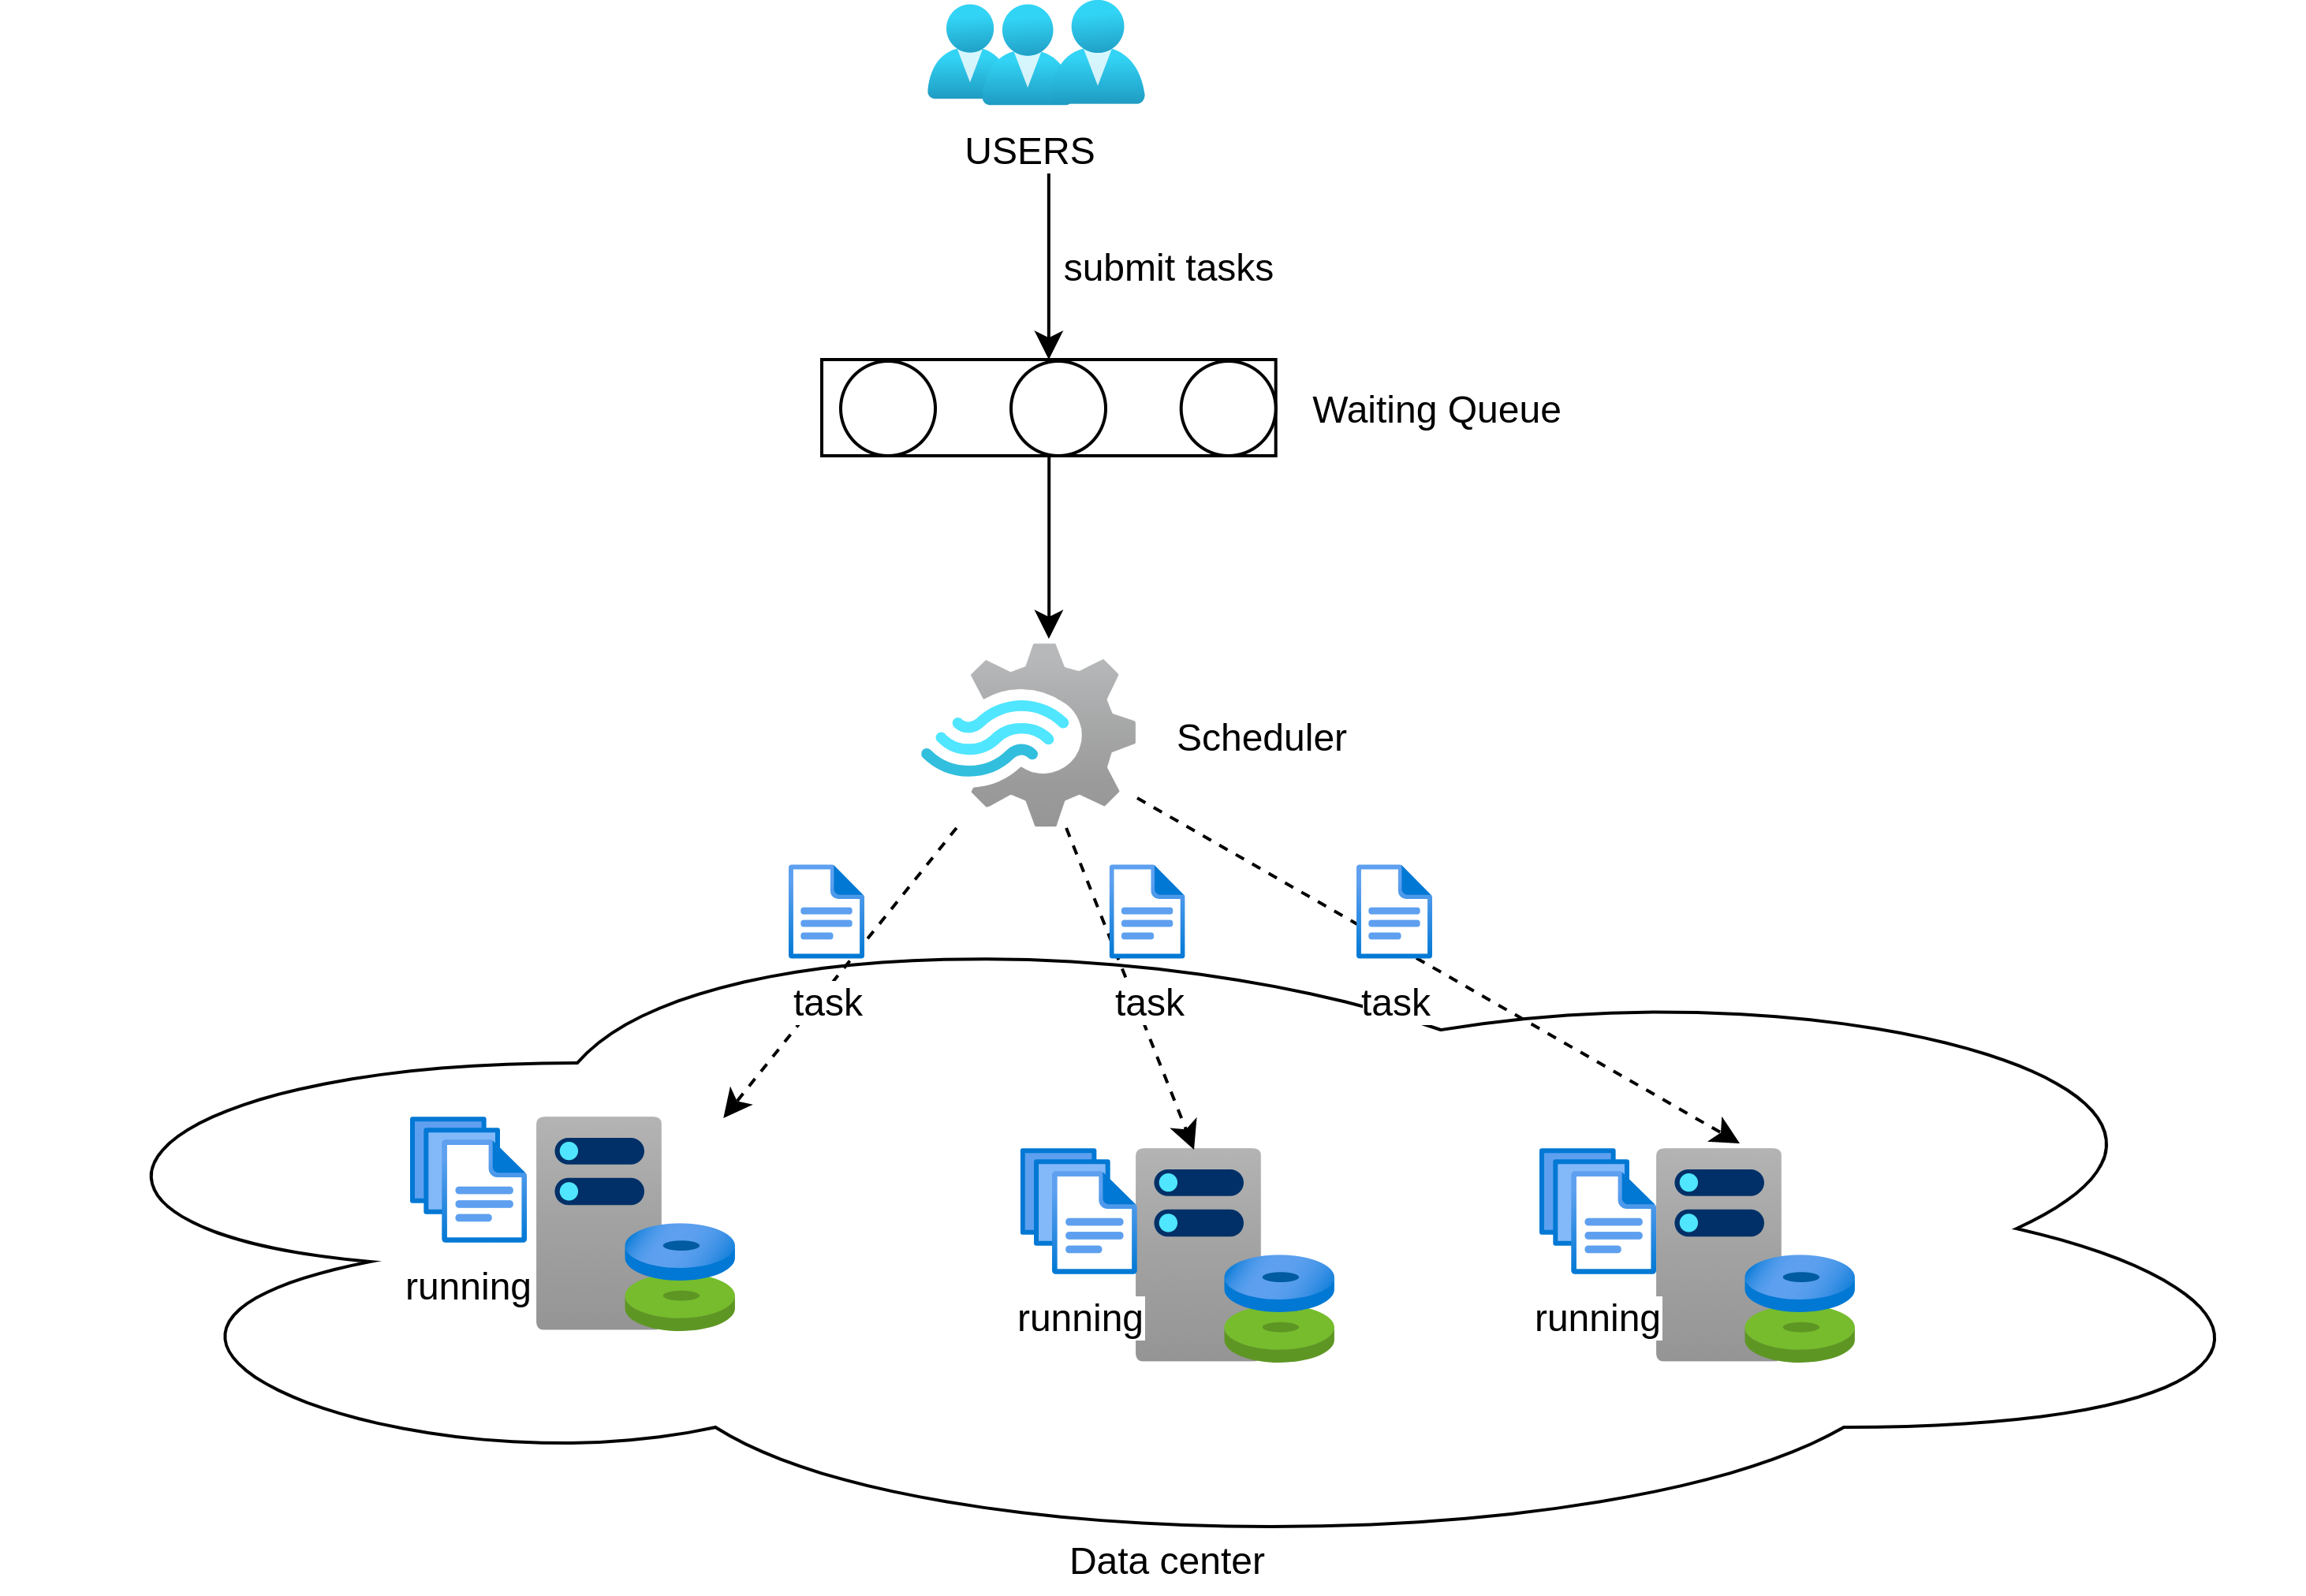
\includegraphics[scale=0.4]{images/basic_flow.png}
		\caption{Người dùng gửi tasks đến hệ thống}
	\end{figure}
\end{minipage}
\end{frame}



\begin{frame}
\frametitle{Giới thiệu bài toán}

\begin{block}
{Bài toán lập lịch}
Lập lịch là quá trình gán các jobs, tasks được yêu cầu tới các máy tính thích hợp để thực thi, hoặc tạo các máy tính ảo từ tài nguyên vật lý để hoàn thành công việc. \\[1cm]
\end{block}

Có hai mức trong bài toán lập lịch 
\begin{itemize}
    \item \textbf{Virtual Machine Level}: Task được gán và thực thi trên các máy ảo bằng chương trình lập lịch gọi là task scheduler, hay còn là task scheduling.
    \item \textbf{Host Level}: Phân chia các máy tính ảo vào các phần cứng, quá trình này gọi là Virtual Machine Scheduling. 
\end{itemize}
\begin{block}
{Sau đây ta sẽ tập chung vào phần Task Scheduling.}
\end{block}
\end{frame}

\begin{frame}

\begin{minipage}[t]{0.48\linewidth}
\begin{block}{Bài toán lập lịch}
\begin{itemize}
    \item \textbf{Virtual Machine Level}: Task được gán và thực thi trên các máy ảo bằng chương trình lập lịch gọi là task scheduler, hay còn là task scheduling.
    \item \textbf{Host Level}: Phân chia các máy tính ảo vào các phần cứng, quá trình này gọi là Virtual Machine Scheduling. 
\end{itemize}
\end{block}
\end{minipage}
\hfill
\begin{minipage}[t]{0.48\linewidth}
	\begin{figure}
		\centering
		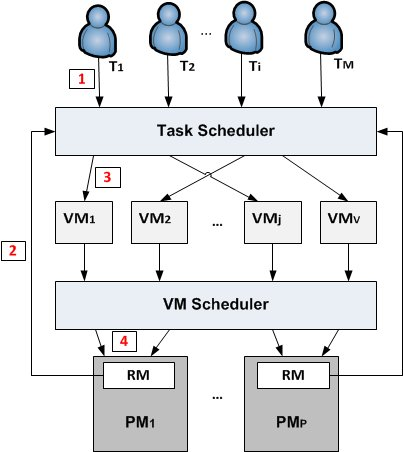
\includegraphics[scale=0.3]{images/scheduling_types.jpg}
	\end{figure}
\end{minipage}
\end{frame}

\subsection{Lập lịch trong môi trường Cloud Computing}

\begin{frame}
{Lập lịch thời gian thực trong môi trường Cloud Computing}

\begin{block}
{Lập lịch thời gian thực}
Trong mô trường thực tế, các tasks đến với hệ thống theo dạng luồng liên tục, số lượng tasks là vô hạn. 
\end{block}

\begin{block}
{Mô hình}
\begin{itemize}
	\item $vms = \{vm_{1}, vm_{2}, ..., vm_{M}\}$ là tập M vector thông tin của máy ảo
	\item $tasks = \{task_{1}, task_{2}, ..., task_{N}\}$ là tập vector thông tin của tasks với $N \to \infty$
	\item $times = \{t_{1}, t_{2}, ..., t_{N}\}$ là tập thời gian đến hệ thống của các task 
	\item $constraints = \{r_{1}, r_{2}, ..., r_{N}\}$ là tập ràng buộc ứng với các task 
\end{itemize}
\end{block}
\end{frame}

\begin{frame}
{Các kiểu tasks}


\begin{block}
{Các tasks này sẽ được chia thành 2 loại: }
\begin{itemize}
	\item \textit{long-run}: các công việc mà không có thời điểm kết thúc, luôn chạy để xử lý những nhu cầu ngắn hạn của người dùng. Ví dụ: Gmail, Docs, web search, ...
	\item \textit{batch-job}: các công việc có thời gian chạy cụ thể, thường từ vài giây đến vài ngày, dao động tùy thuộc vào hiệu năng của hệ thống. Ví dụ: người dùng gửi đến công việc huấn luyện một mô hình học máy, hoặc chạy một script phân tích dữ liệu, ... 
\end{itemize}
\end{block}
\end{frame}

\begin{frame}
{Vấn đề}

\begin{block}
{\centering Trạng thái của task ảnh hưởng đến trạng thái hệ thống}
\begin{figure}[h!]
    \centering
    \subfloat[\centering Luồng hoạt động của hệ thống]{{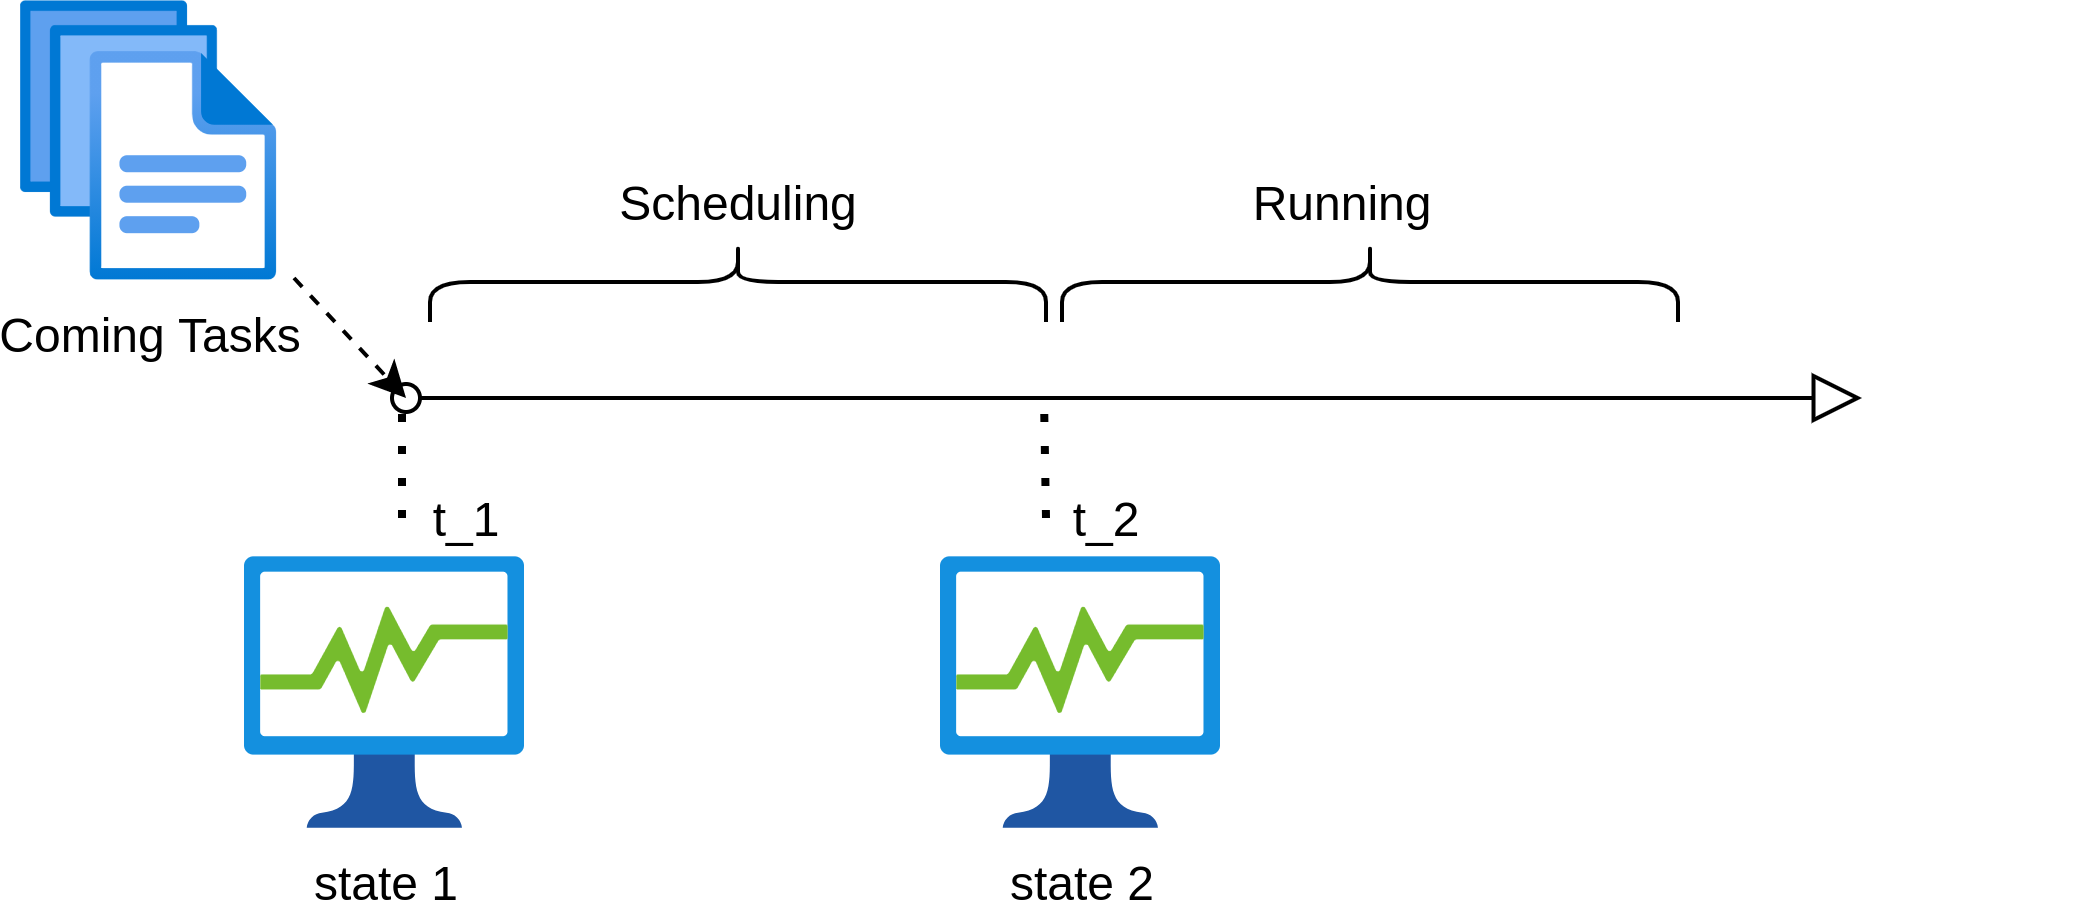
\includegraphics[width=4cm]{images/state_change.png} }}%
    \qquad
    \subfloat[\centering Trạng thái của task]{{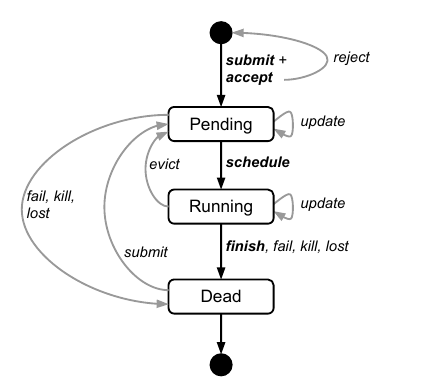
\includegraphics[width=4cm]{images/task_states.png} }}%
\end{figure}
\end{block}
\end{frame}

\begin{frame}
{Vấn đề}

\begin{block}
{Trạng thái của task làm mất cân bằng phân phối tài nguyên giữa các máy ảo}
\begin{figure}[h!]
    \centering
    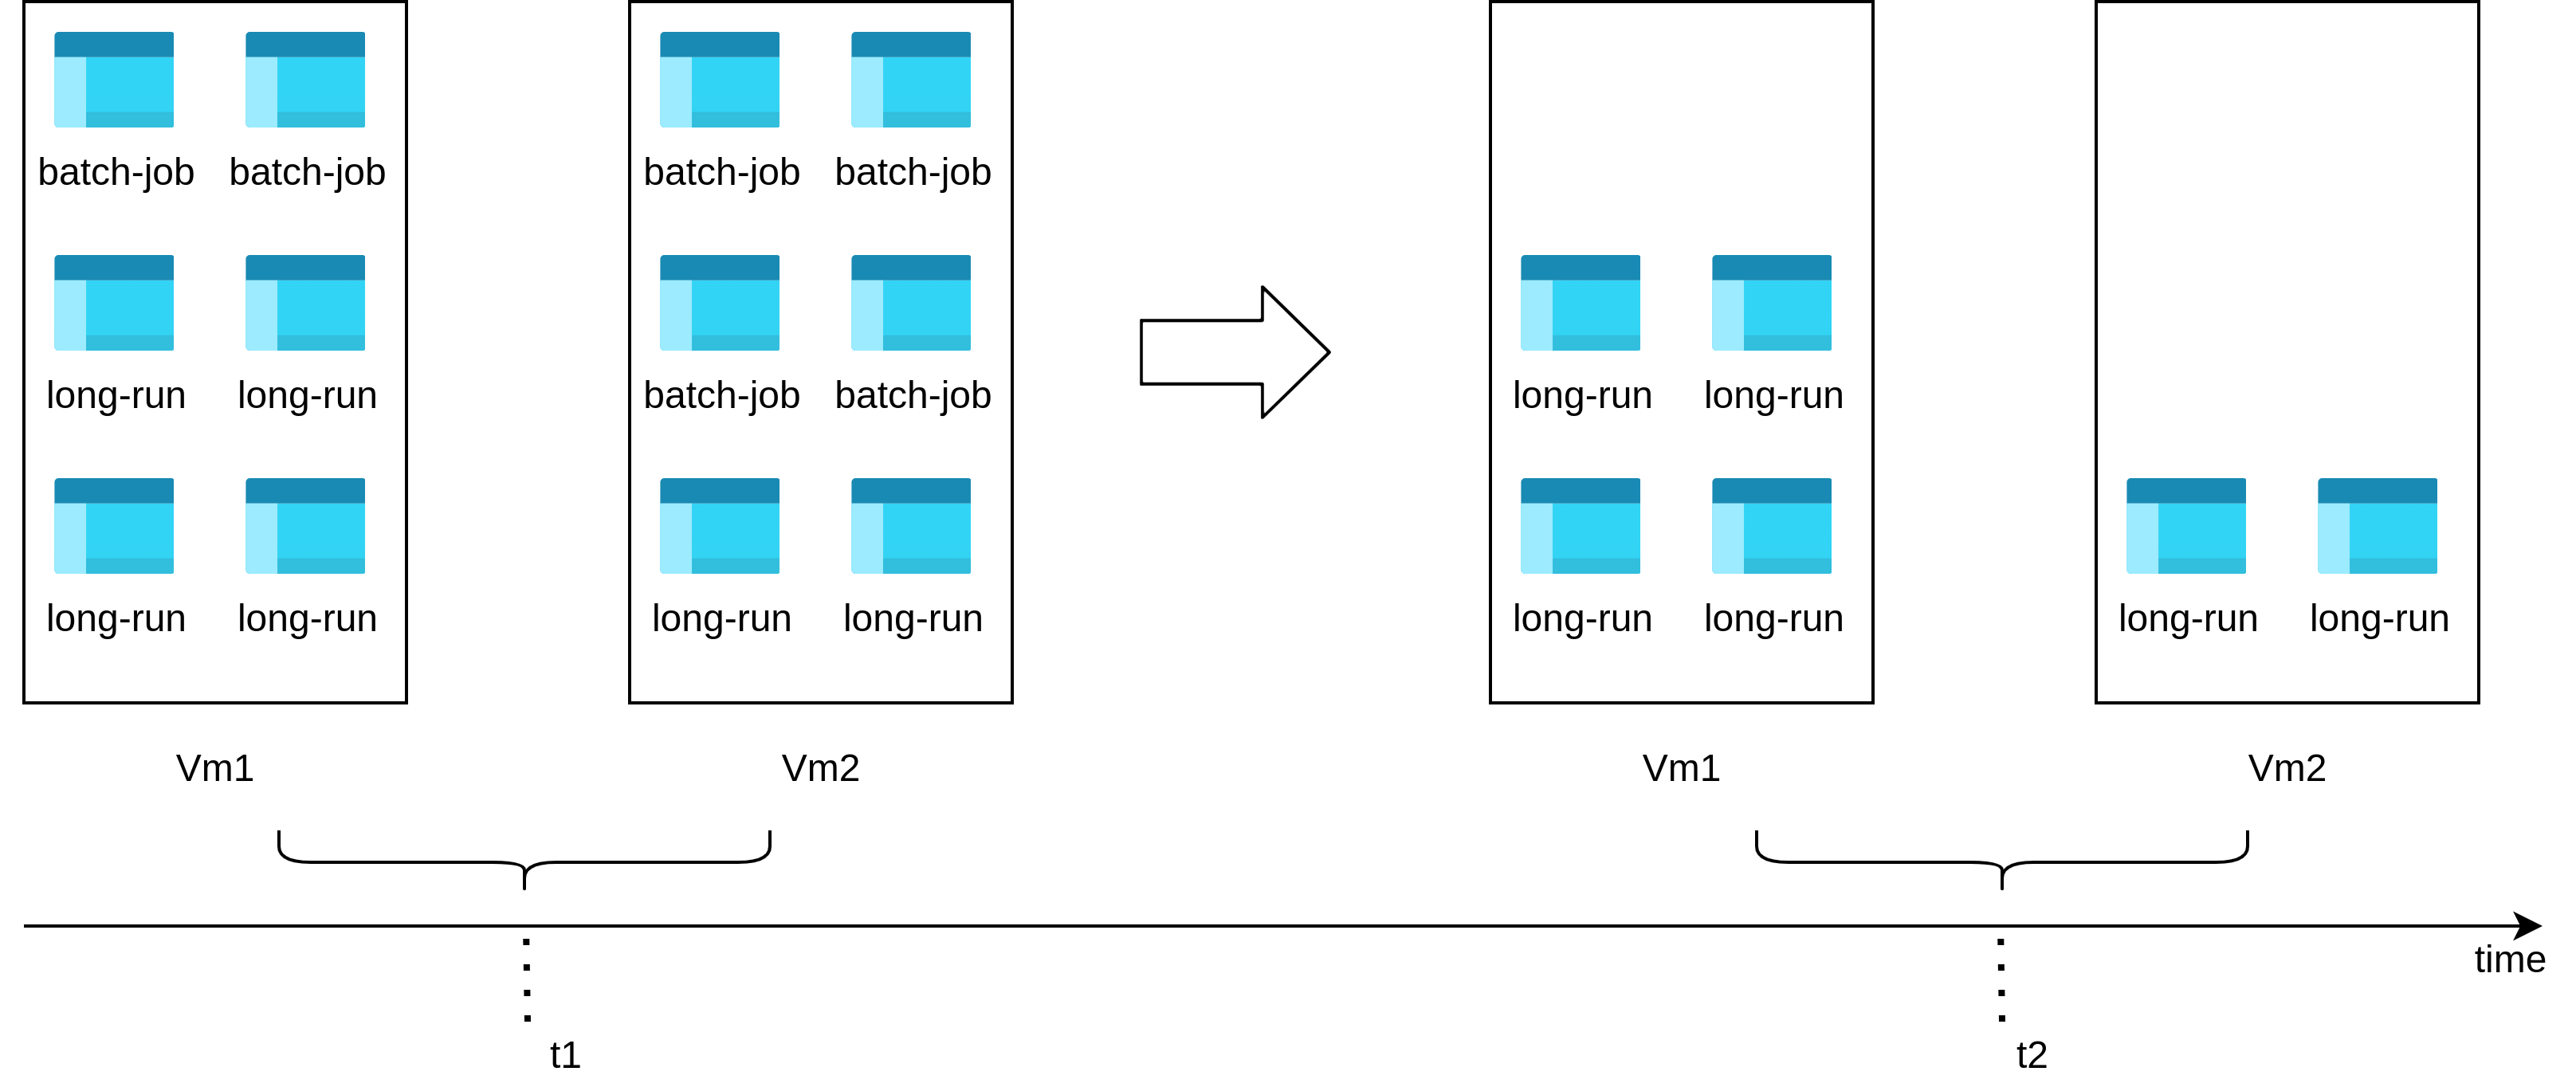
\includegraphics[scale=0.5]{images/unload_balancing.png}
\end{figure}
\end{block}
\end{frame}

\section{Mô hình lập lịch đề xuất}

\begin{frame}
{Mô hình lập lịch đề xuất}

\begin{block}
{\centering Mô hình hoạt động}
\begin{figure}
	\centering
	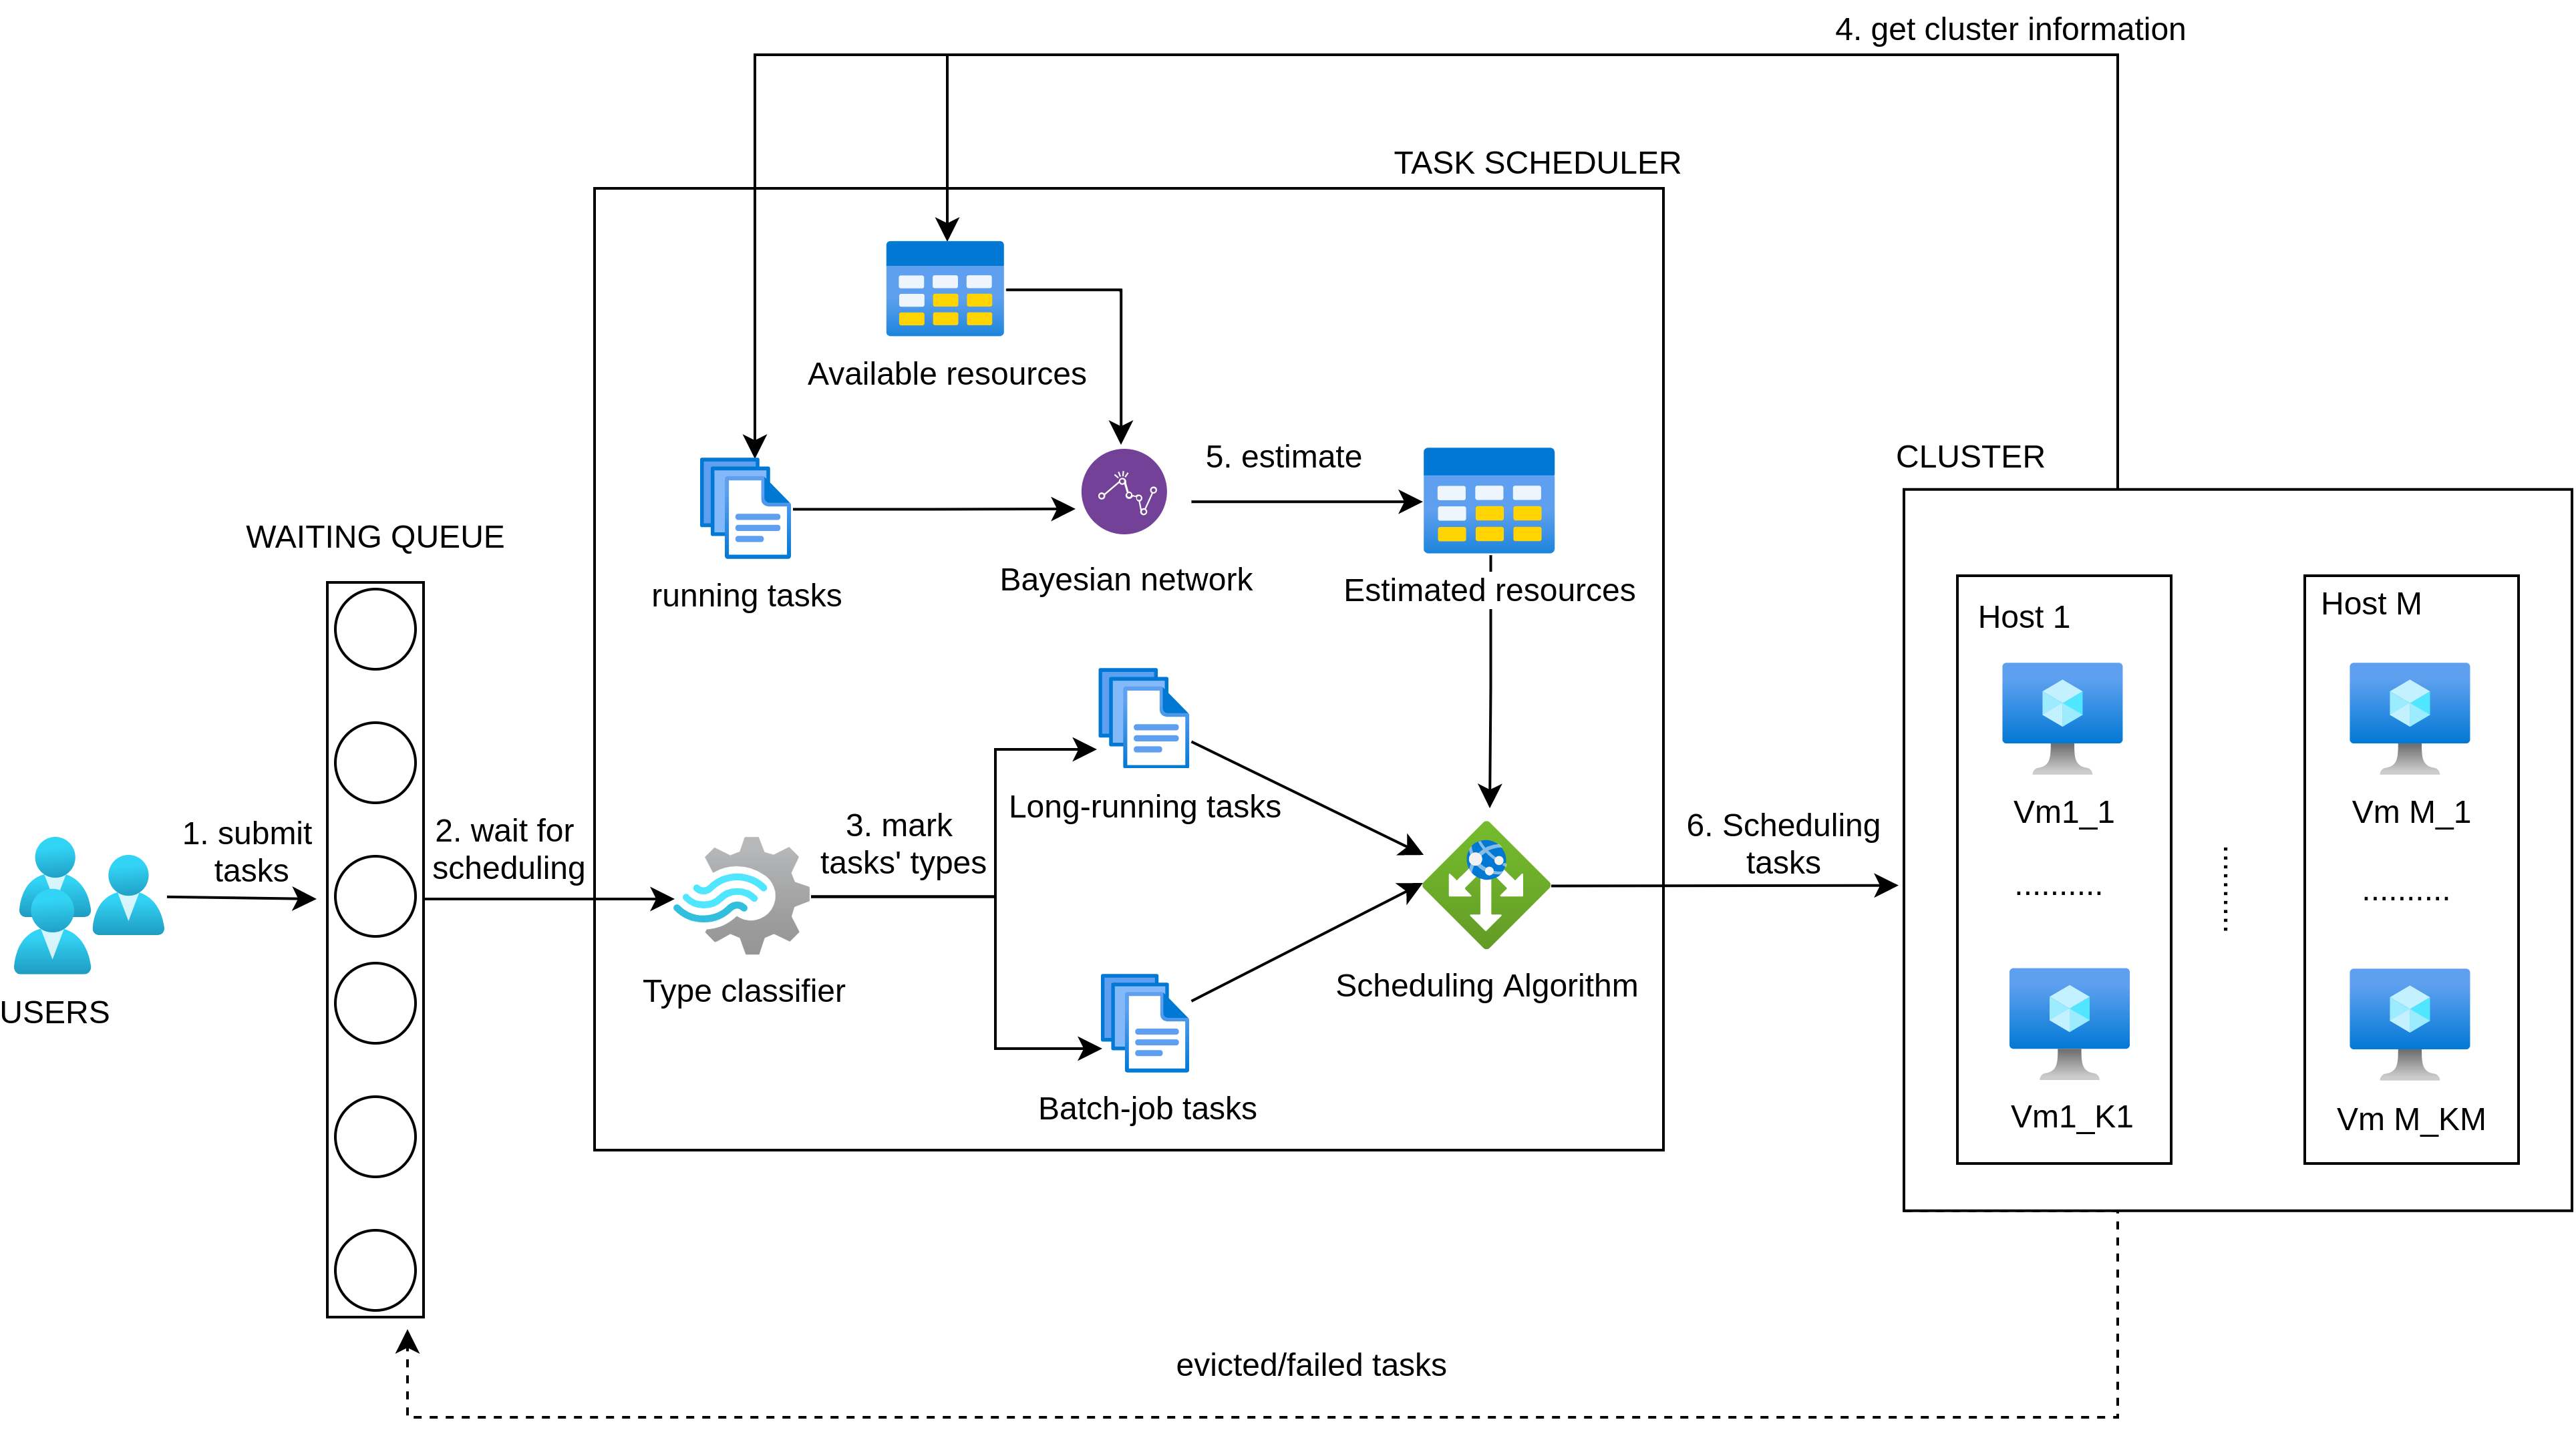
\includegraphics[scale=0.4]{images/system_flows.png}	
\end{figure}
\end{block}
\end{frame}

\begin{frame}
	\begin{minipage}[t]{0.4\linewidth}
		\begin{block}{Luồng hoạt đông}
		\begin{itemize}
			\item <1-> \textbf{1.} Người dùng gửi các công việc đến hệ thống, được chuyển đến hàng đợi cho việc lập lịch
			\item <2-> \textbf{2.} Các tasks chờ đợi đến khi đủ số lượng hoặc vượt quá một khoảng thời gian cố định 
		\end{itemize}
		\end{block}
	\end{minipage}
	\hfill
	\begin{minipage}[t]{0.59\linewidth}
		\begin{figure}
			\centering
			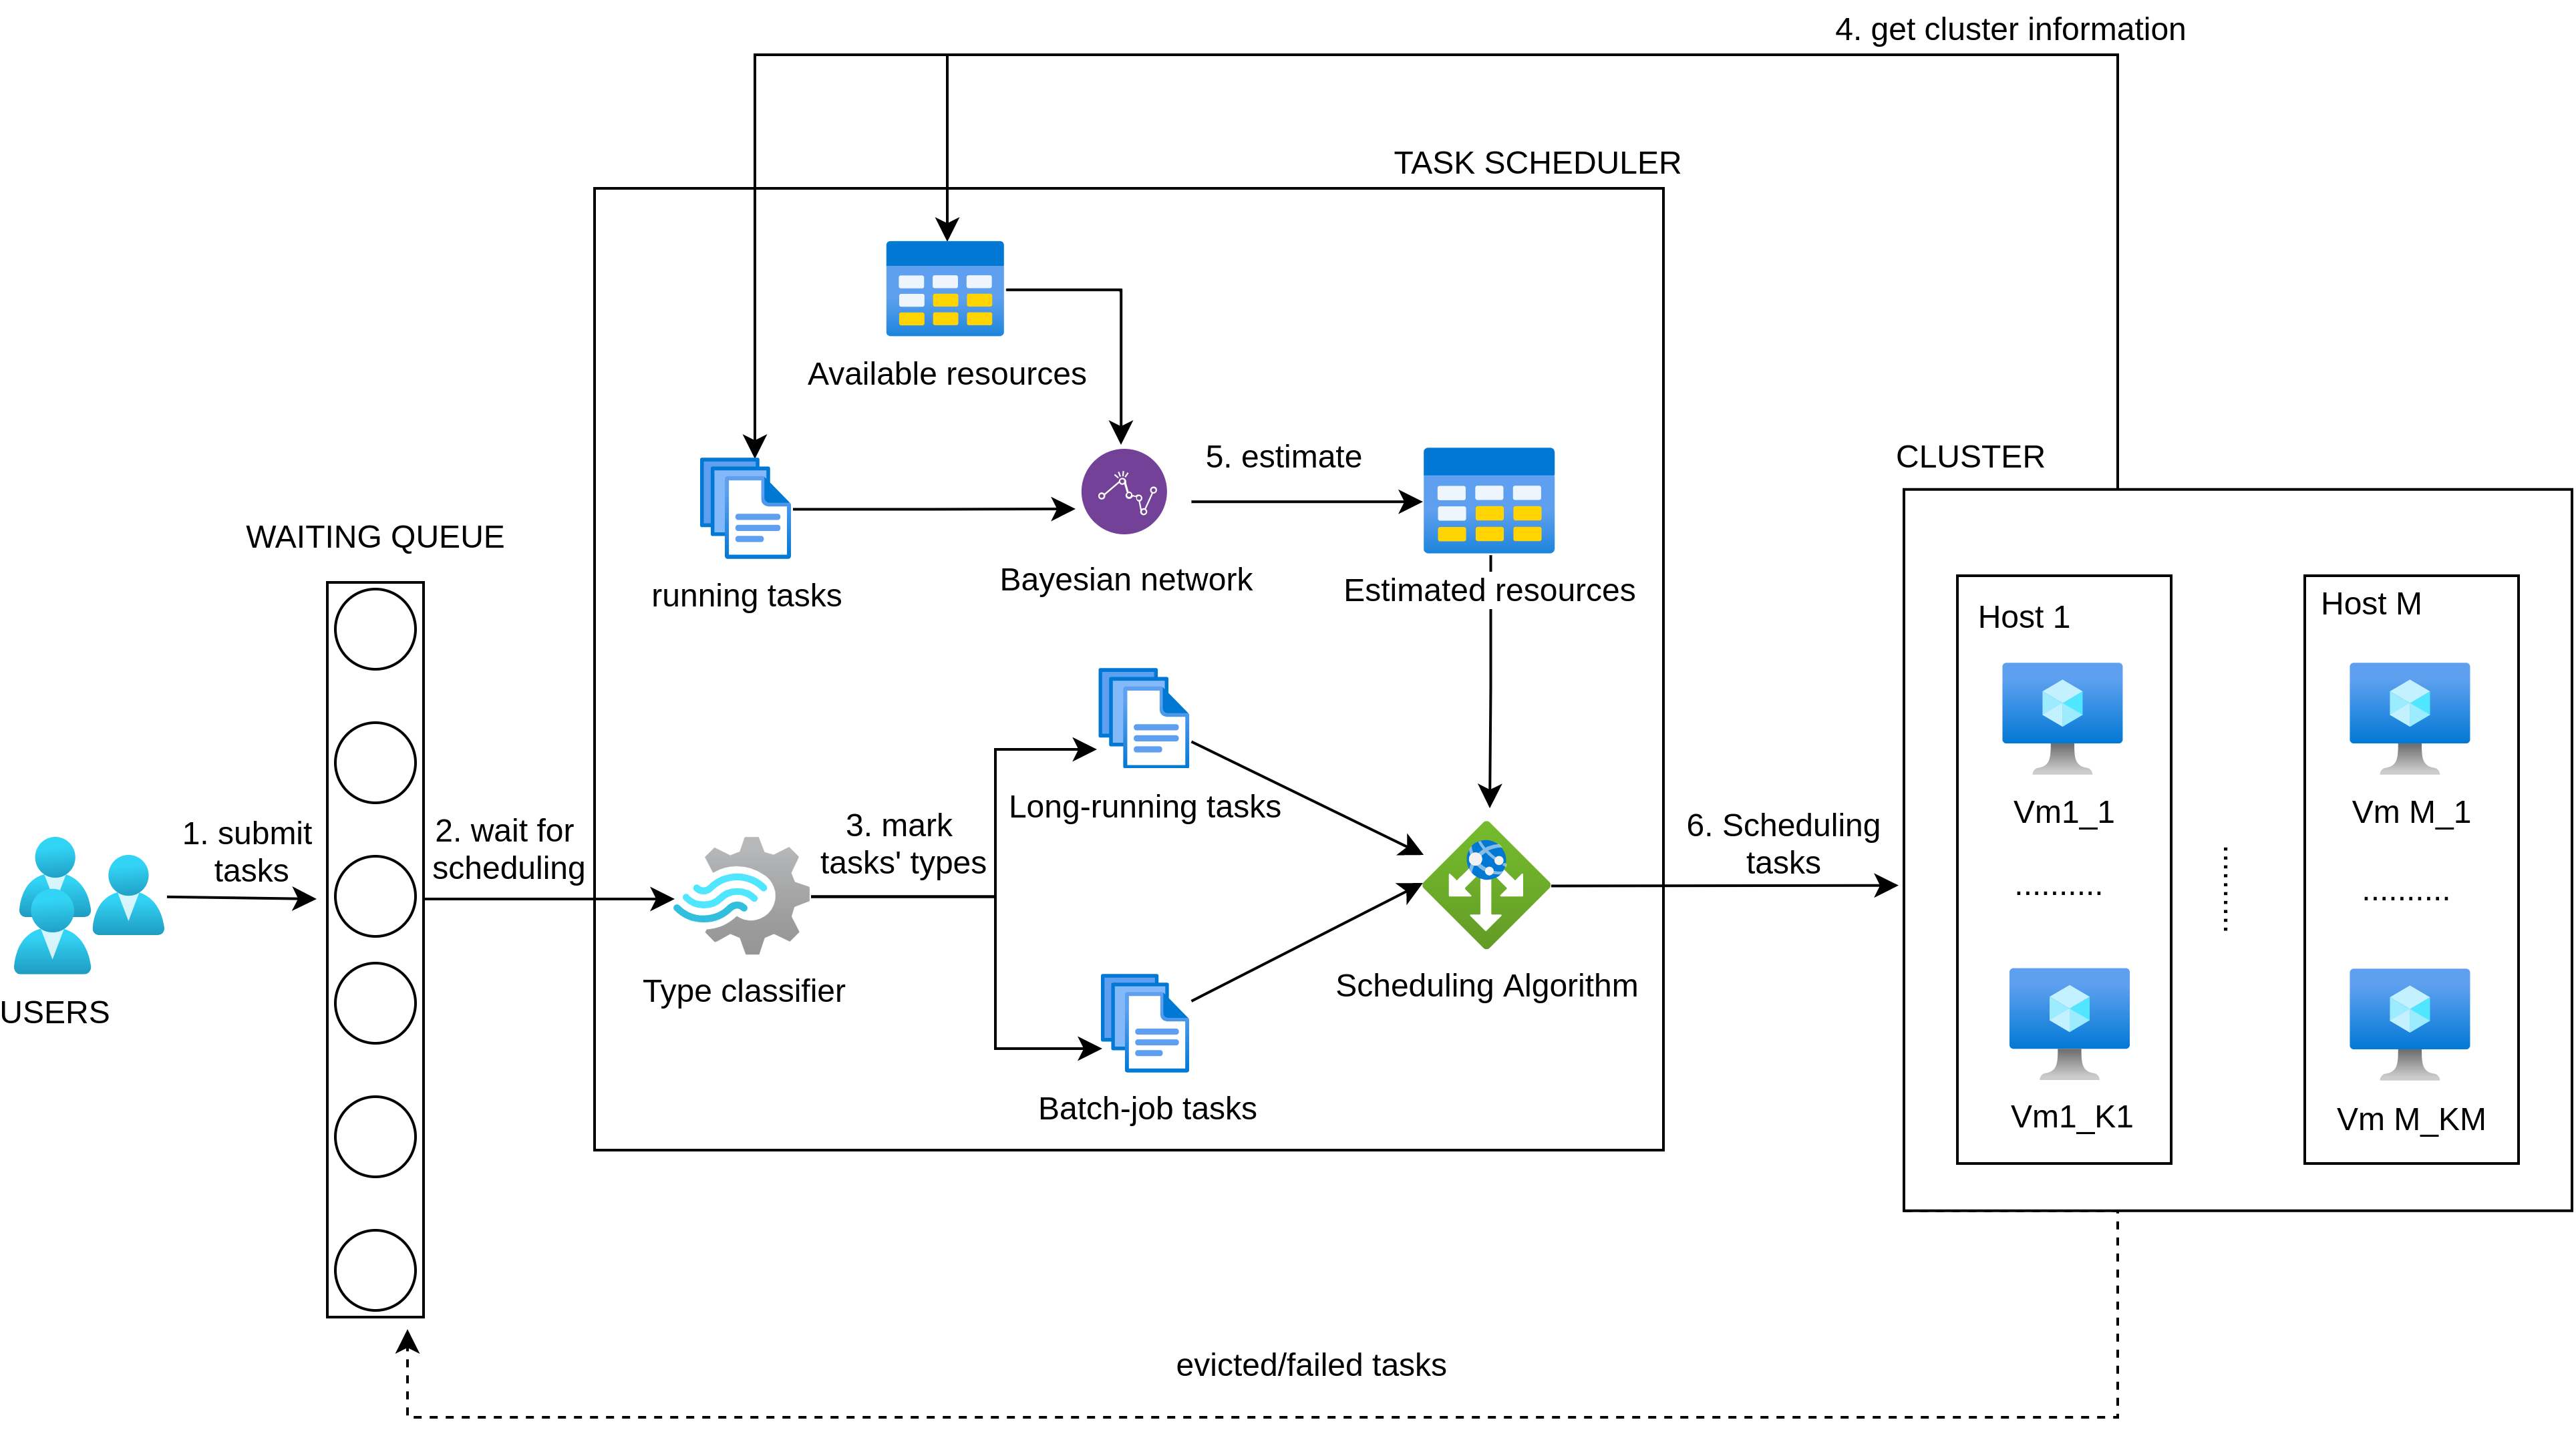
\includegraphics[scale=0.3]{images/system_flows.png}
			\caption{Mô hình đề xuất}
		\end{figure}
	\end{minipage}
\end{frame}

\begin{frame}
	\begin{minipage}[t]{0.5\linewidth}
	\begin{block}{Luồng hoạt động}
		\begin{itemize}
			\item <1-> \textbf{3.} Dựa vào thông tin metadata của tasks, ta phân loại công việc thành 2 kiểu là long-running và batch-job
			\item <2-> \textbf{4.} Bộ lập lịch lấy các thông tin về trạng thái hệ thống, bao gồm các tasks đang được chạy trong hệ thống và thông tin về tài nguyên của các máy tính ảo  
		\end{itemize}
		\end{block}
	\end{minipage}
	\hfill
	\begin{minipage}[t]{0.49\linewidth}
		\begin{figure}
			\centering
			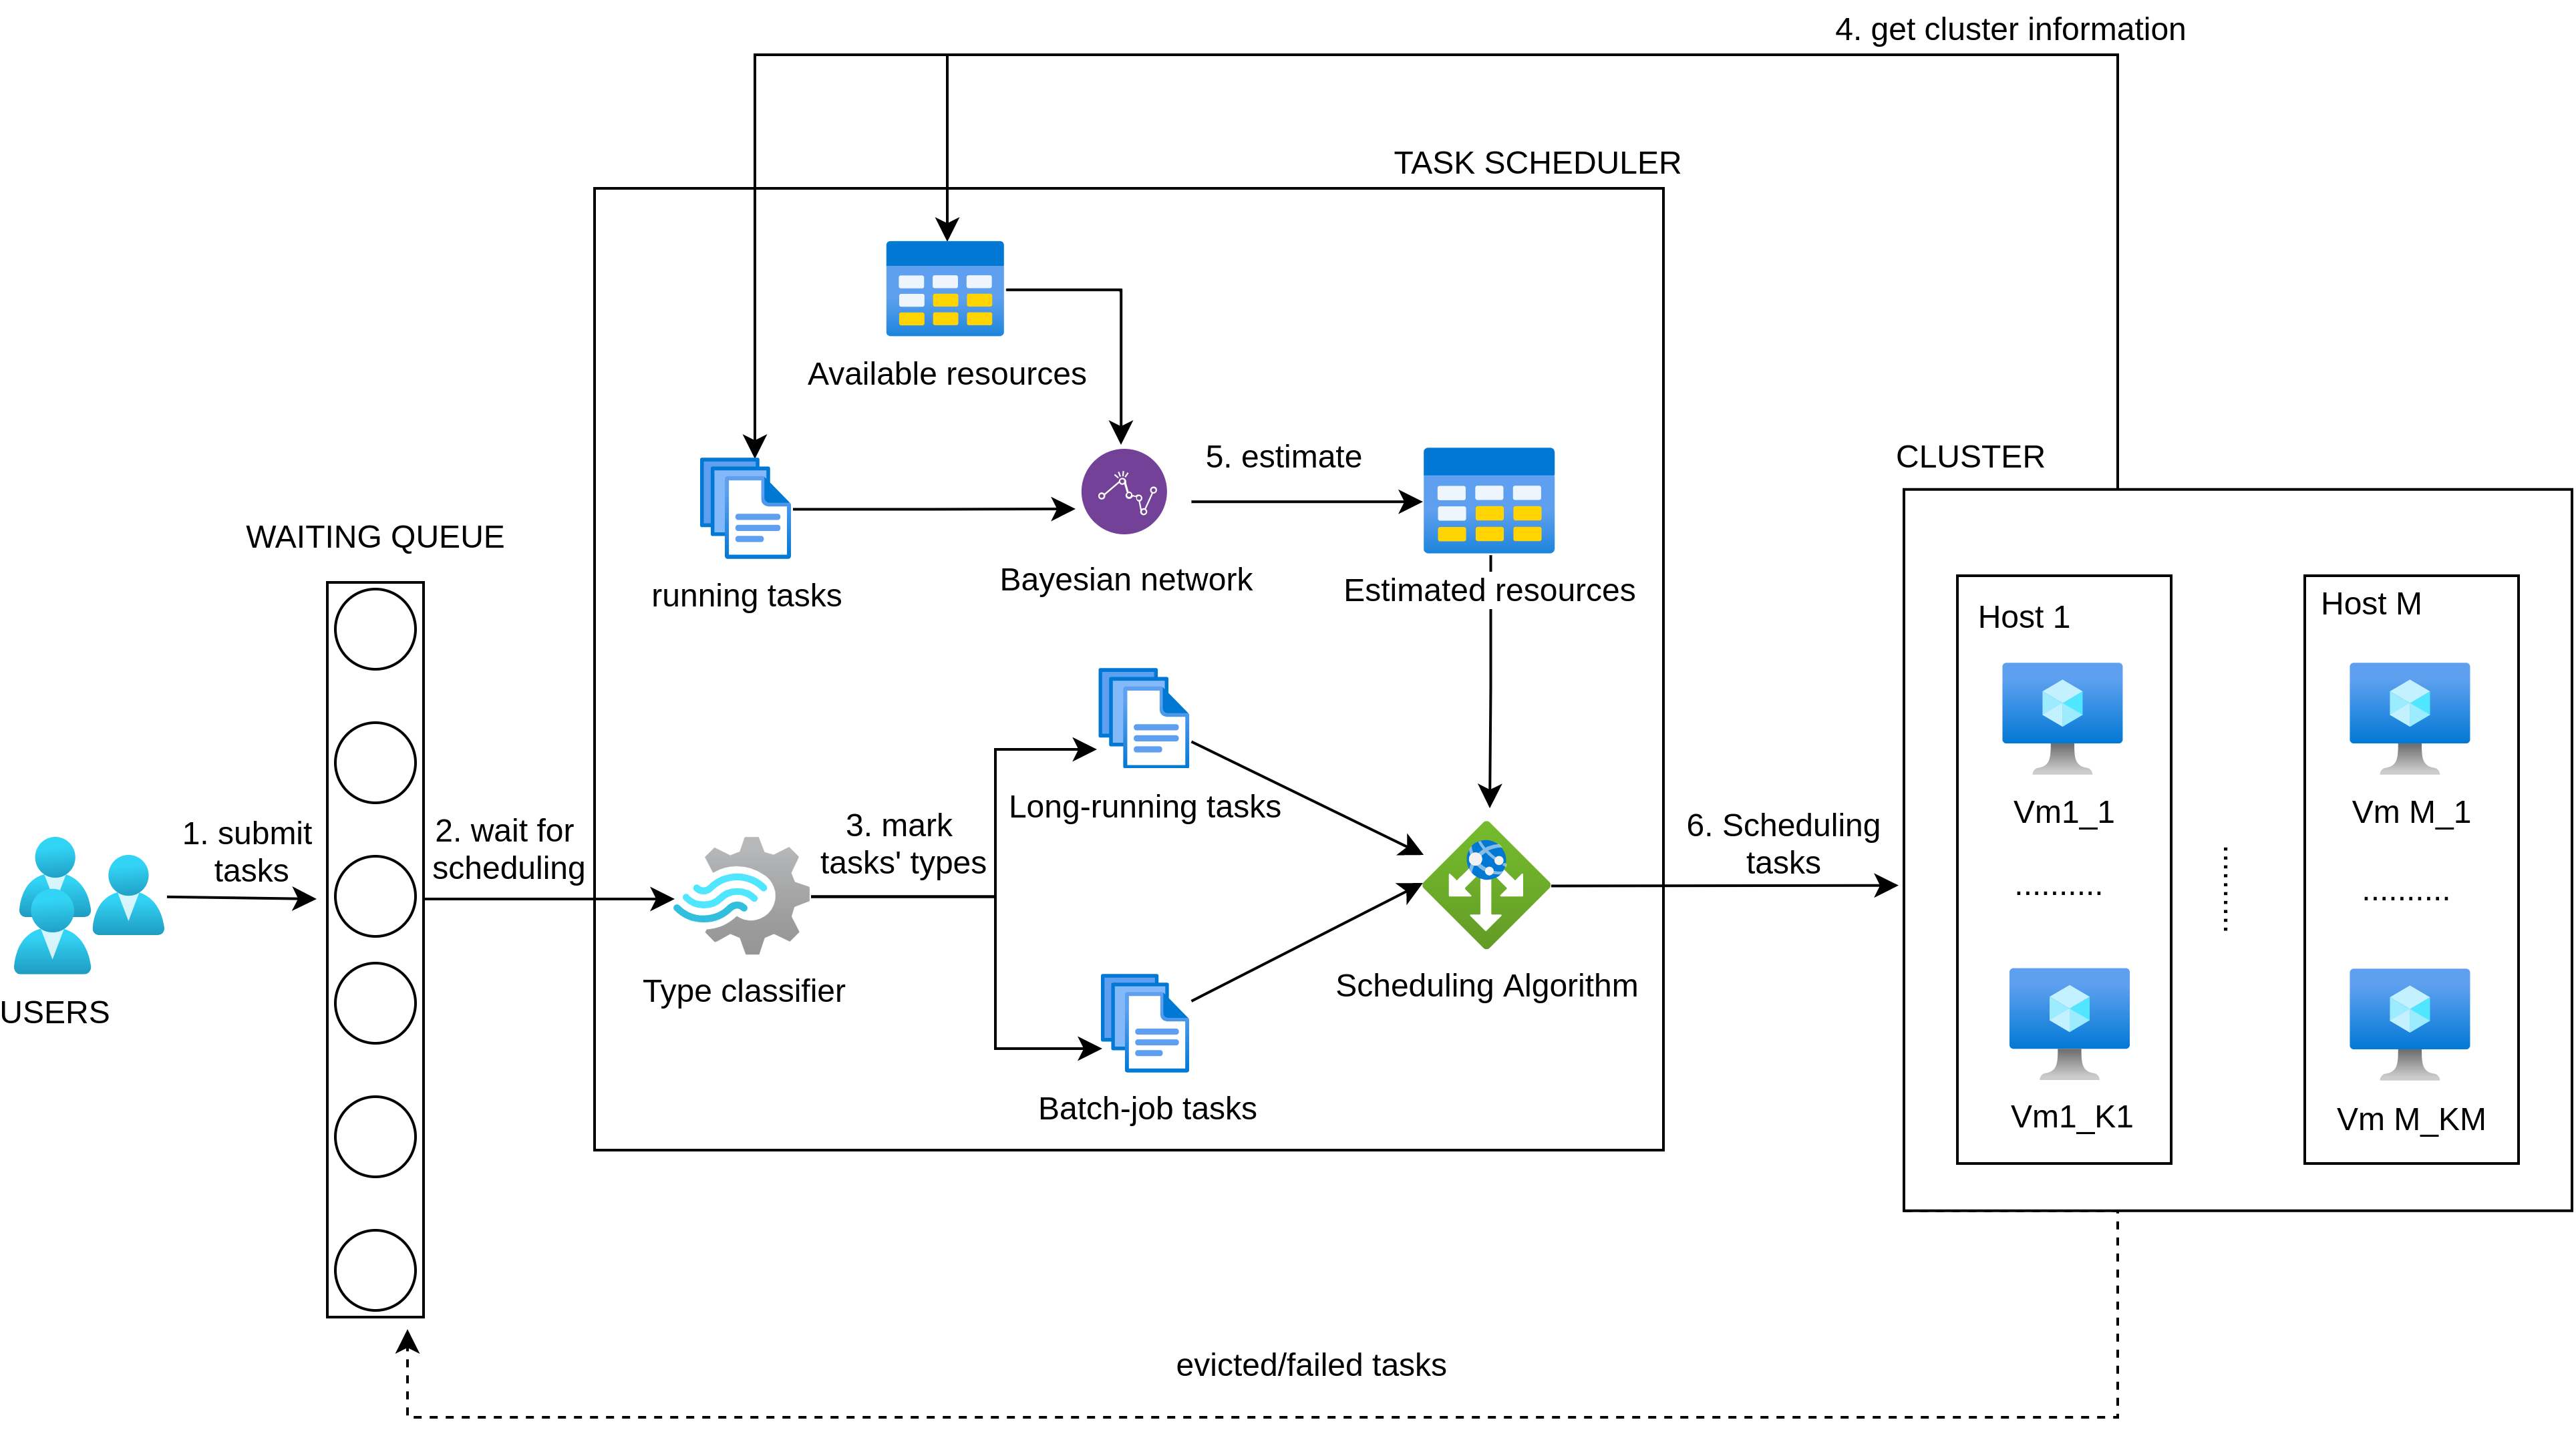
\includegraphics[scale=0.25]{images/system_flows.png}
			\caption{Mô hình đề xuất}			
		\end{figure}
	\end{minipage}
\end{frame}

\begin{frame}
	\begin{minipage}[t]{0.4\linewidth}
	\begin{block}{Luồng hoạt động}
		\begin{itemize}
			\item <1-> \textbf{5.} Sử dụng mạng Bayesian để ước lượng tài nguyên khả dụng tại thời điểm tasks được thực thi trên các máy ảo 
			\item <2-> \textbf{6.} Lập lịch cho các tasks với thông tin tài nguyên ước lượng
		\end{itemize}
	\end{block}
	\end{minipage}
	\hfill
	\begin{minipage}[t]{0.59\linewidth}
		\begin{figure}
			\centering
			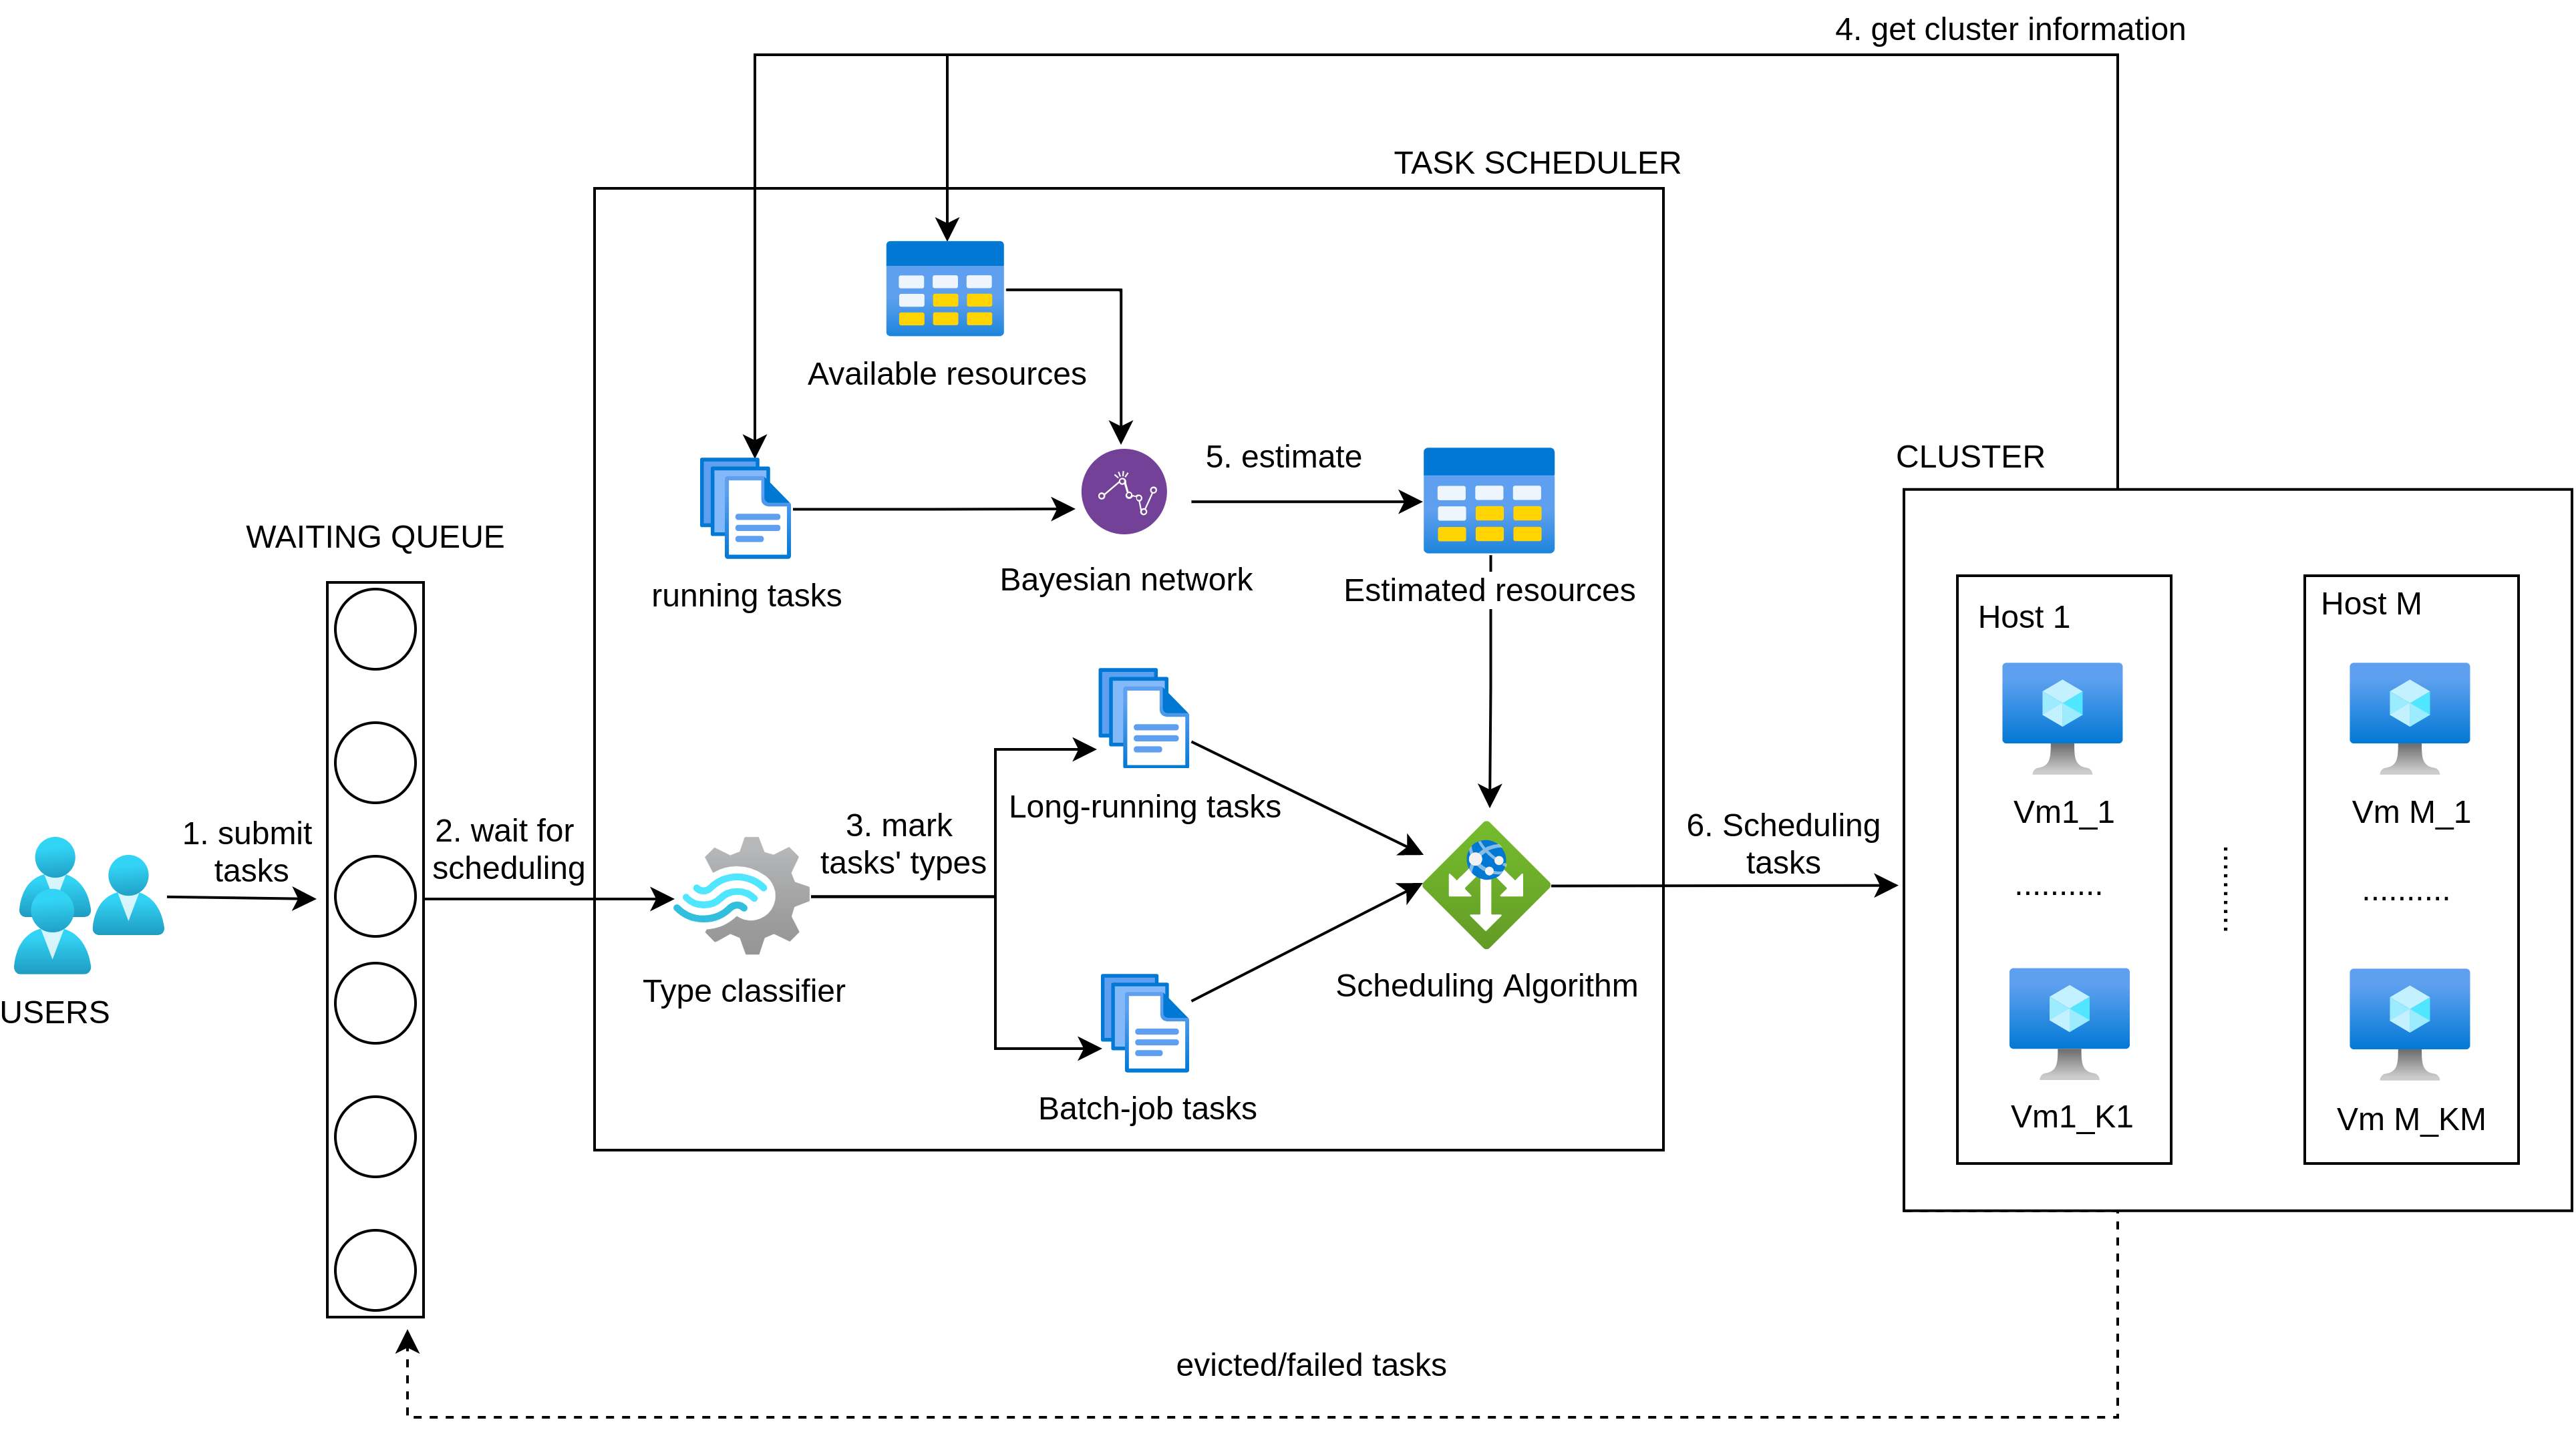
\includegraphics[scale=0.3]{images/system_flows.png}
			\caption{Mô hình đề xuất}
		\end{figure}
	\end{minipage}
\end{frame}


\subsection{Bayesian Network For Estimating Task's Status}

\begin{frame}
{Biểu diễn mạng}
\begin{figure}[h!]
	\centering 
	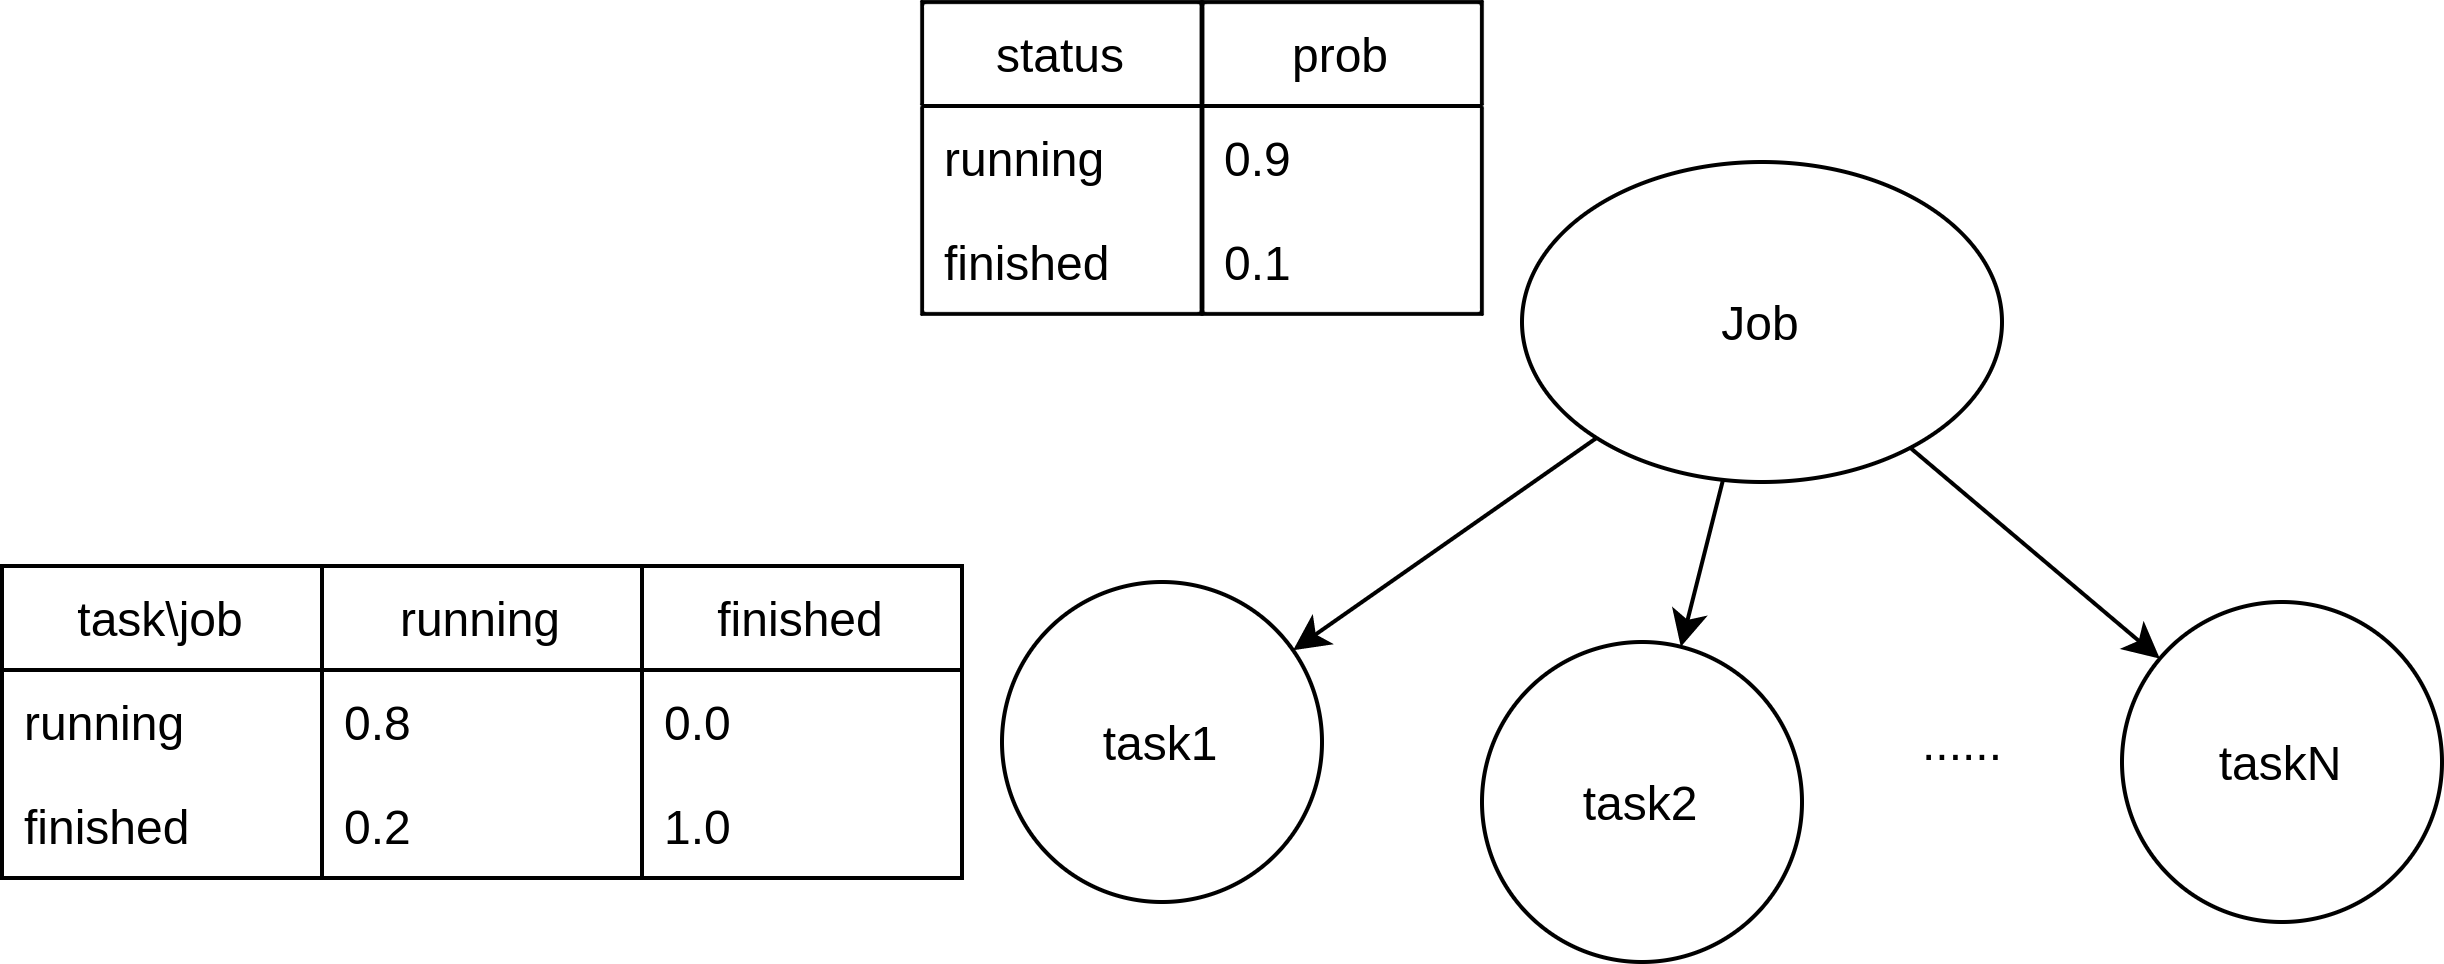
\includegraphics[scale=0.6]{images/job_network.png}
	\caption{Mạng Bayesian thể hiện quan hệ giữa các tasks trong cùng một job}
	\label{fig:job_network}
\end{figure}
\end{frame}

\begin{frame}
{Suy diễn}
\begin{figure}[h!]
	\centering 
	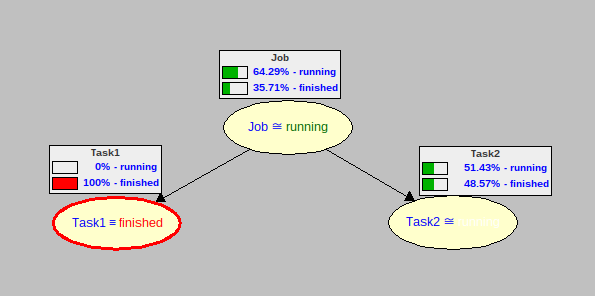
\includegraphics[scale=0.6]{images/task_finished_observation.png}
	\caption{Suy diễn khi quan sát một task kết thúc}
	\label{fig:job_network}
\end{figure}
\end{frame}

\section{Experiments and results}

\begin{frame}
{Thông tin về dữ liệu}

\begin{table}[h!]
	\centering
        \begin{tabular}{| p{1.5cm} | p{1.5cm} | p{1.5cm} | p{1.5cm} |}
            \hline
            \multicolumn{4}{|c|}{Tasks' description} \\
            \hline
            stats & cpu & memory & storage \\
            	 & request (\%) & request (Mb) & request (Mb) \\
            \hline 
            \hline
            count & 15000 & 15000 & 15000 \\
            \hline
            mean & 0.051 & 24.93 & 11.0 \\
            \hline
            std & 0.056 & 40.35 & 5.2 \\
            \hline
            min & 0.006 & 1.24 & 0.1 \\
            \hline 
            25\% & 0.025 & 20.39 & 12.6 \\
            \hline 
            50\% & 0.025 & 26.75 & 12.6 \\
            \hline
            75\% & 0.313 & 26.75 & 12.6 \\
            \hline 
            max & 0.251 & 101.91 & 63.2 \\
            \hline
        \end{tabular}
\end{table}
\end{frame}

\begin{frame}
{Số liệu so sánh về thời gian}
\begin{table}[h!]
	\centering
	\caption{Kết quả về thời gian chạy của các tasks}
	\begin{tabular}{|p{1.5cm}| p{1.5cm} | p{1.5cm} | p{1.6cm}|}
		\hline
		\multicolumn{4}{|c|}{Running statistics over 1000s} \\
		\hline
		stats & FCFS & Worstfit & Resources \\
			&	&	& balancing \\
		\hline
		\hline
		count&13214&13925&14235 \\
		\hline
		mean&10.62&6.34&5.42 \\
		\hline
		std&54.24&33.37&27.31 \\
		\hline
		min&0.31&0.12&0.21 \\
		\hline
		25\%&3.15&2.09&2.08 \\
		\hline
		50\%&5.78&3.52&3.41 \\
		\hline
		75\%&8.13&5.61&5.50 \\
		\hline
		max&829.92&616.35&640.39 \\
		\hline
	\end{tabular}
	\label{table:finished_tasks}
\end{table}
\end{frame}

\begin{frame}
{So sánh độ chính xác của mạng Bayesian}
\begin{figure}
\centering
\begin{subfigure}{.5\textwidth}
  \centering
  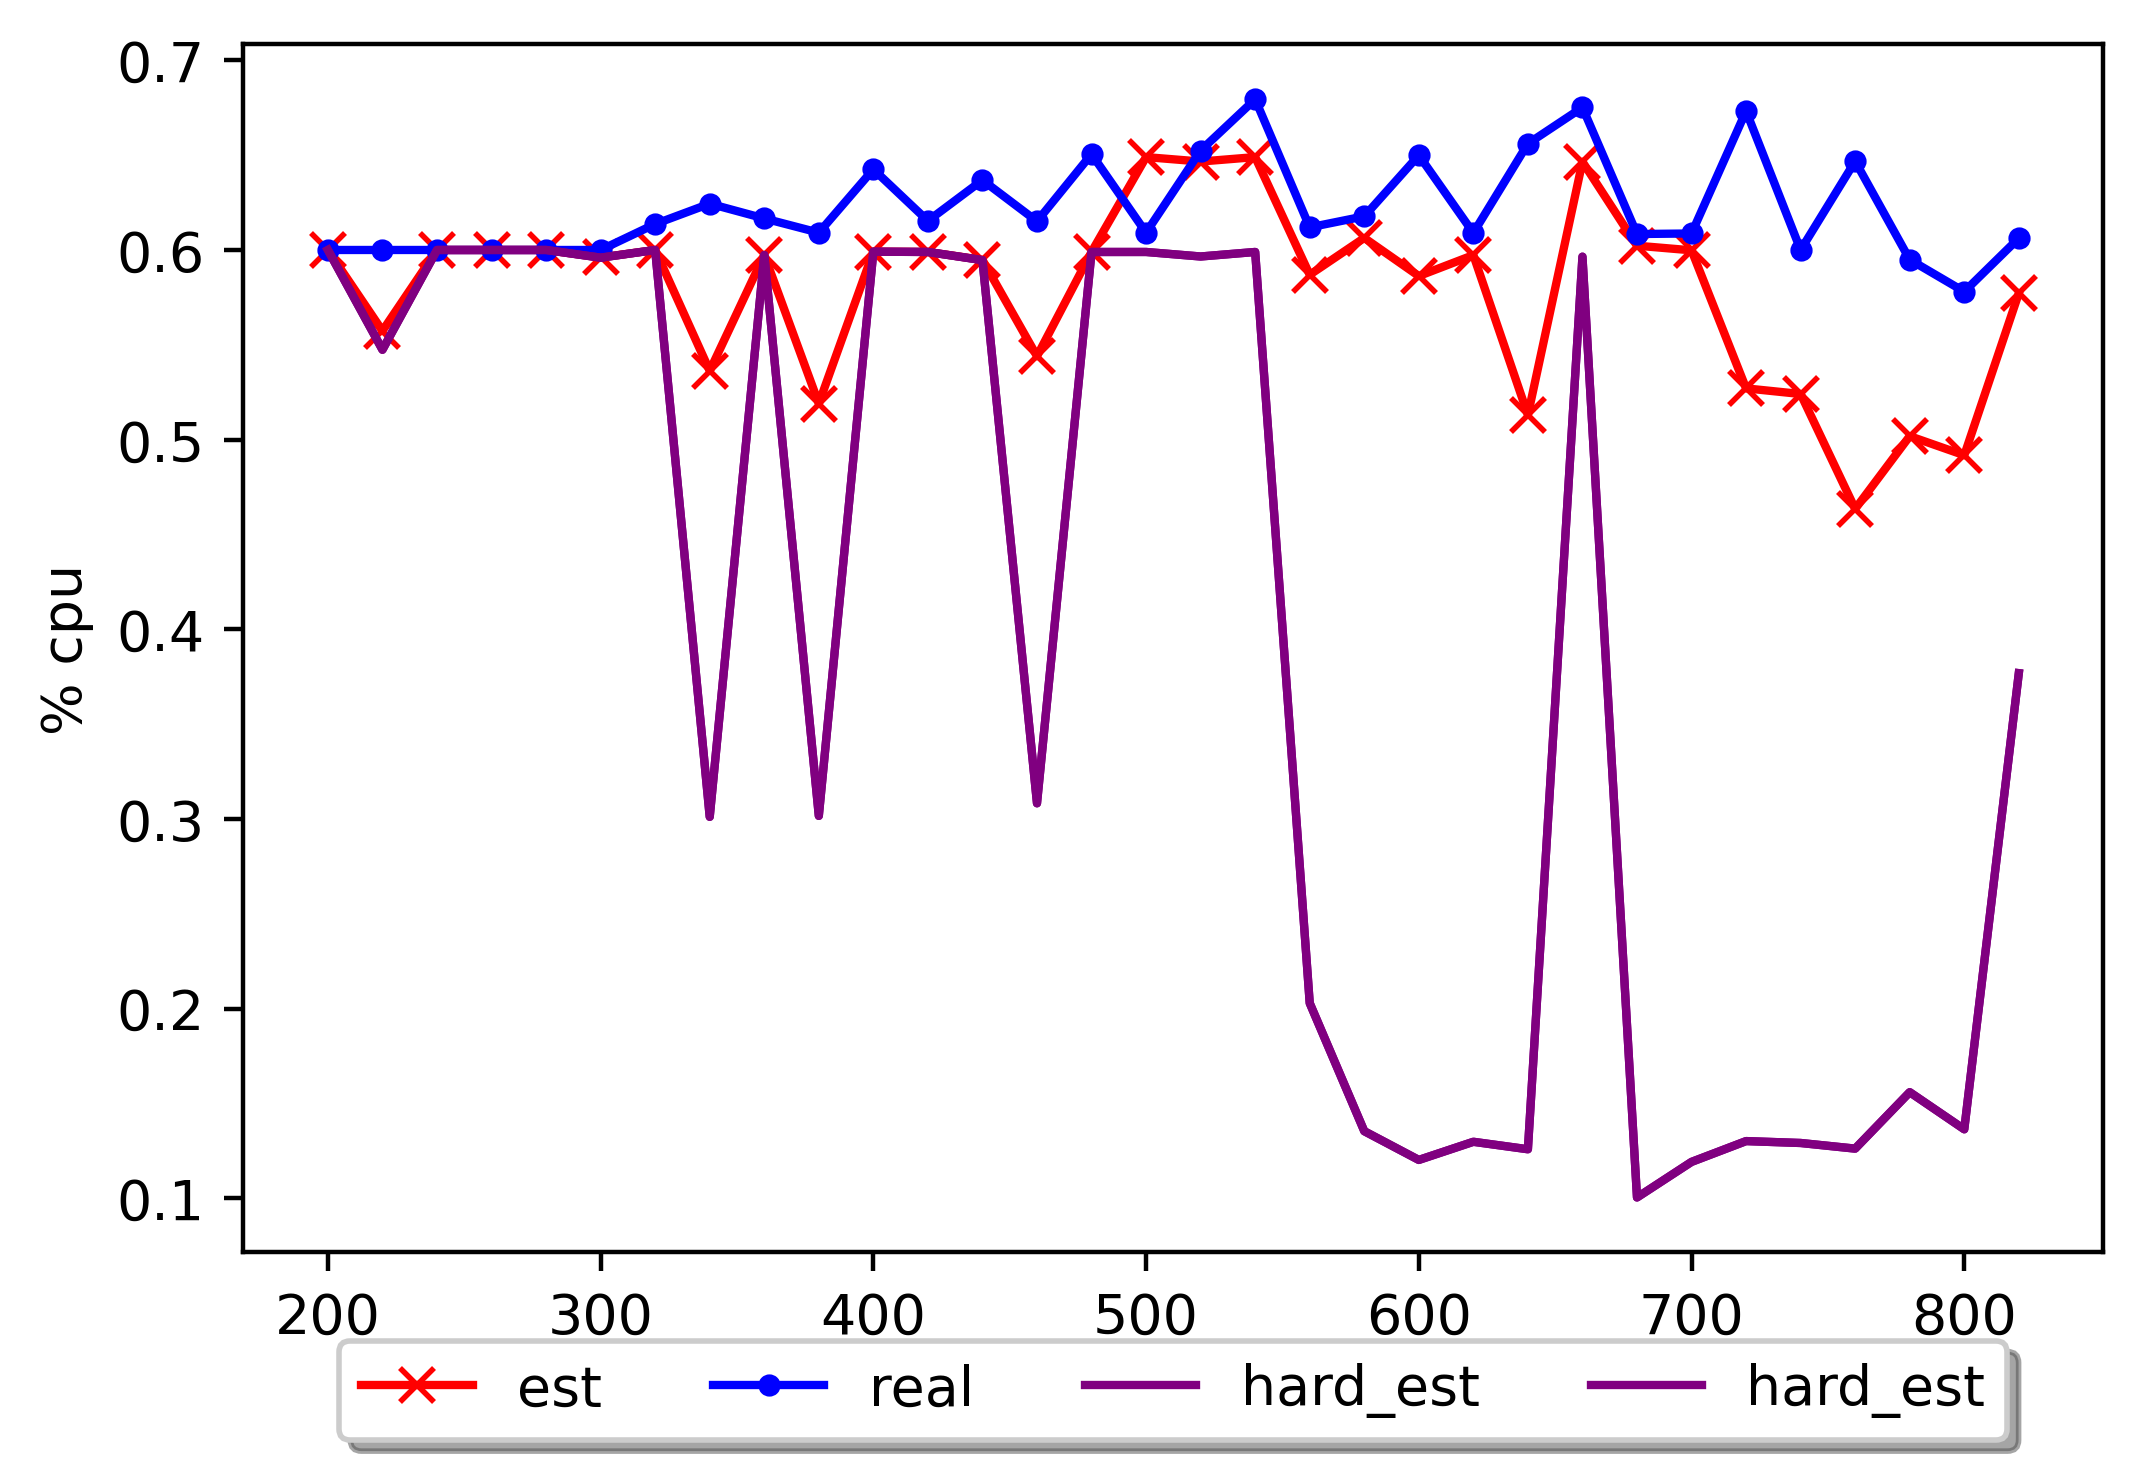
\includegraphics[width=.85\linewidth]{images/cpu_usage_estimation_1.png}
  \caption{Tài nguyên khả dụng tại thời điểm thực thi}
  \label{fig:usage_est_a}
\end{subfigure}%
\begin{subfigure}{.5\textwidth}
  \centering
  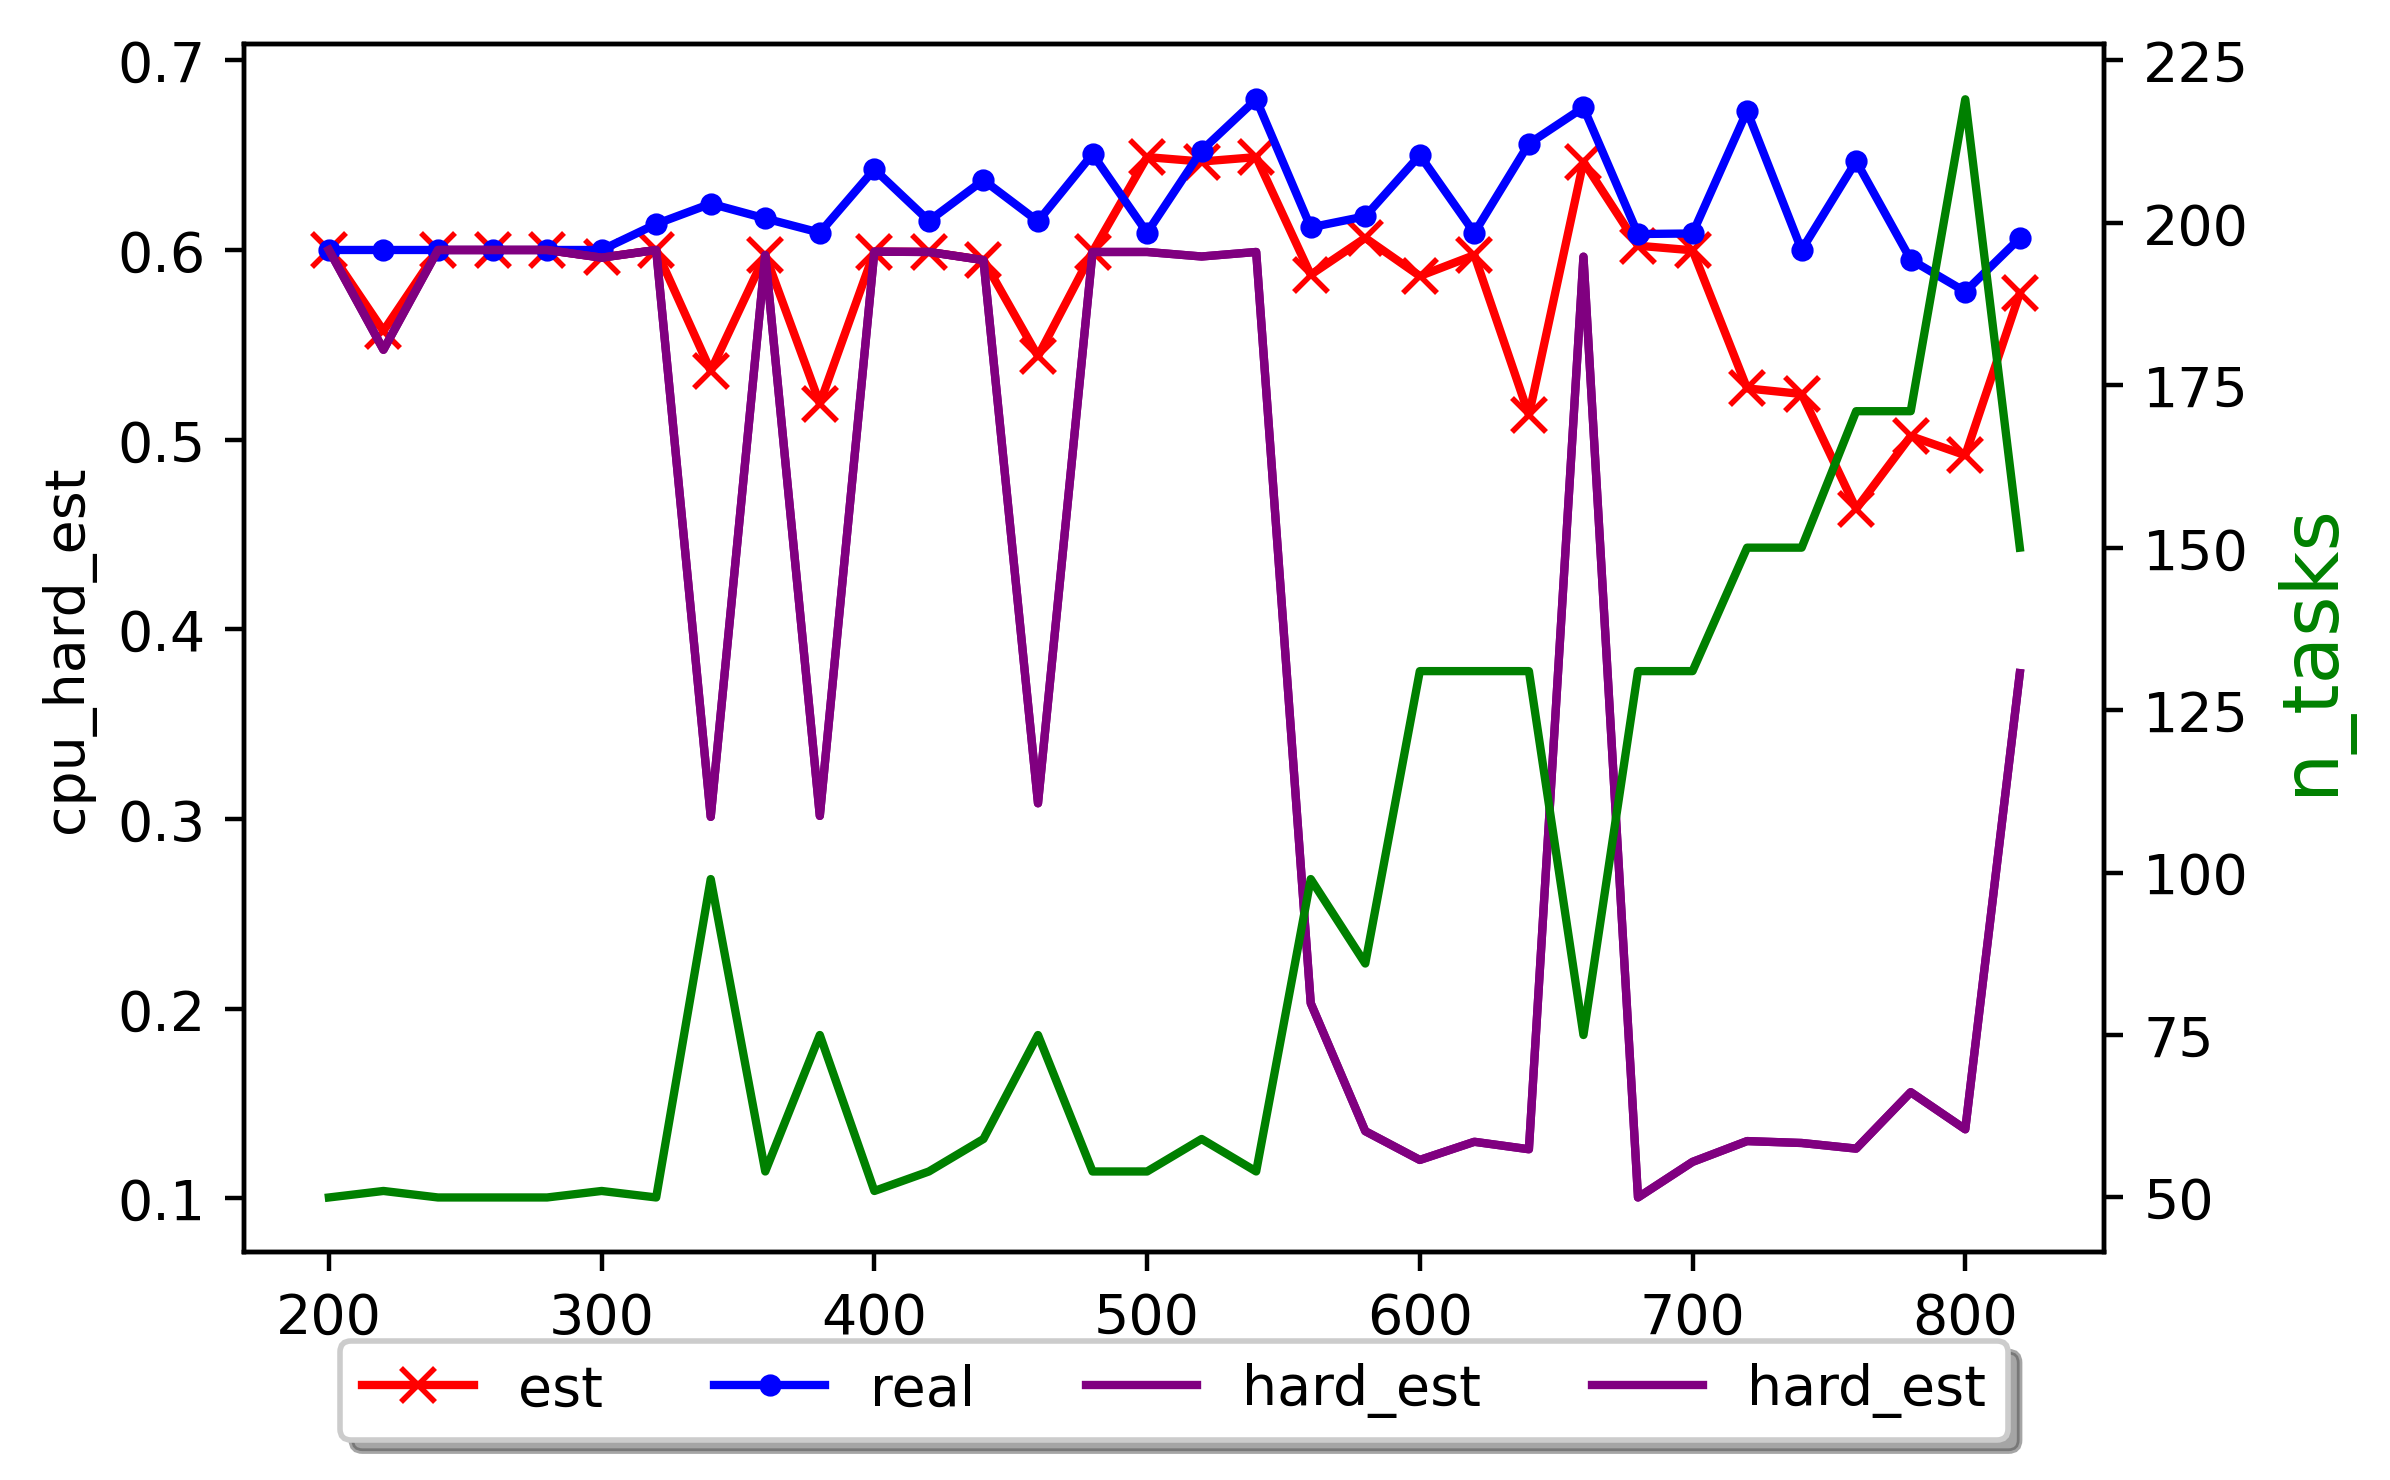
\includegraphics[width=.9\linewidth]{images/cpu_usage_estimation_2.png}
  \caption{Sai số với số lượng tasks đang chạy}
   \label{fig:usage_est_b}
\end{subfigure}
\caption{Thông số tại thời điểm kết thúc lập lịch}
\label{fig:usage_est}
\end{figure}
\end{frame}

\begin{frame}
{So sánh mức độ mất cân bằng giữa các máy tính}
\begin{figure}[h!]
	\centering
	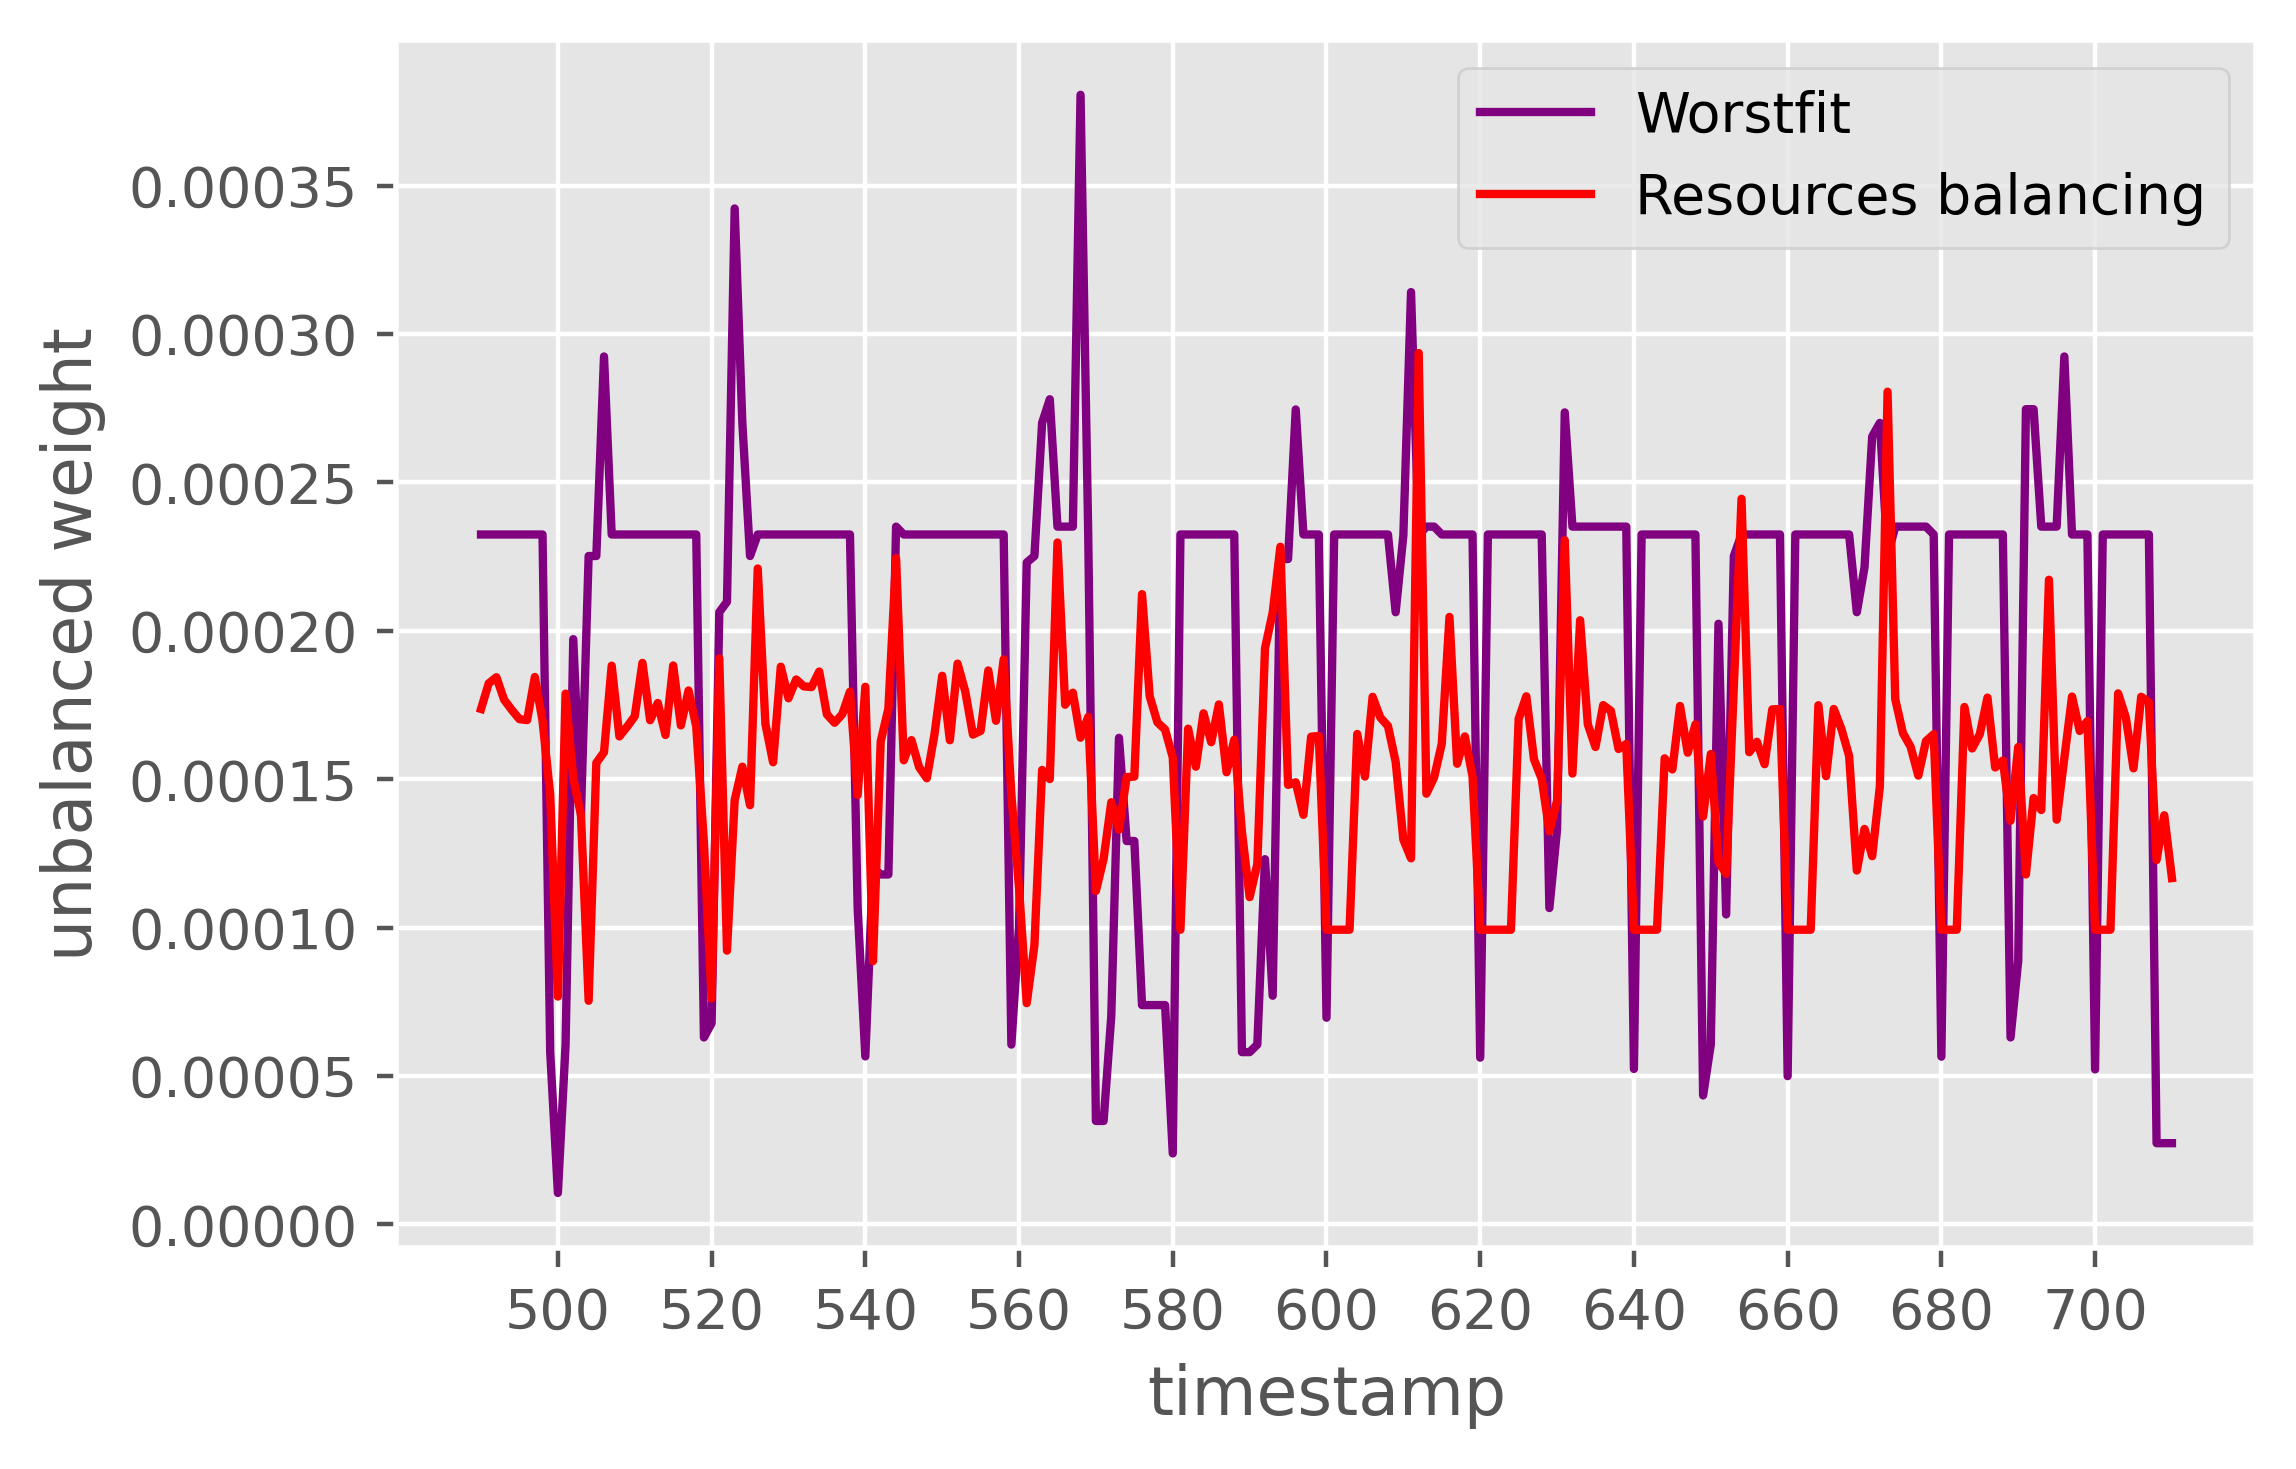
\includegraphics[scale=0.6]{images/unbalanced_weights.png}
	\caption{Mức độ mất cân bằng trong quá trình hoạt động}
\end{figure}
\end{frame}

{\1
\begin{frame}[plain,noframenumbering]
  \finalpage{Thank You For Listening!}
\end{frame}}

\end{document}